\refstepcounter{chapter}
\addcontentsline{toc}{chapter}{Maintenance}

\setsectiontitle{Important Notes}

\subsection*{Lubrication of the Machine}
\begin{itemize}
    \item Lubrication and cooling lubrication of the machine are summarized in the following pages of the operator's manual:
    \begin{itemize}
        \item 7.02-1 \textbf{Machine Lubrication Plan}
        \item 7.03-1 \textbf{Lubrication Regulations}
        \item 7.06-1 \textbf{Lubricant Recommendations}
        \item 7.07-1 \textbf{Coolants}
    \end{itemize}
    \item Lubrication and maintenance of additional equipment are described in Section 6 of the \\operator's manual, categorized by equipment.
    \item The designation of lubricants and their labeling in this manual comply with the new German standard DIN 51 502 (November 1979).
    \item The designation of liquid lubricants follows the ISO viscosity classification based on the kinematic viscosity at 40°C, as specified in DIN 51 519 (July 1976).
    \item The machine lubrication plan (7.02-1) and lubrication regulations (7.03-1) adhere to DIN 8659 (Draft, December 1978).
    \item \textbf{On the machine, oil lubrication nipples are marked in red, while grease nipples are marked with yellow identification discs.} Additionally, identification plates for lubrication nipples and filling points are attached in accordance with DIN 51 502.
\end{itemize}

\subsection*{Lubricants}
\begin{itemize}
    \item A key requirement for operational safety and machine longevity is the use of suitable \\lubricants.
    \item The machine is delivered pre-filled\footnotemark.
    \item The lubricants used for the initial filling (see 7.06-1) should be used continuously. If this is not possible for operational reasons, alternative products from the lubricant \\selection table (7.06-2 and 7.06-3) may be used.
\end{itemize}

\subsection*{Maintenance Tasks}
\begin{itemize}
    \item Apart from lubrication and cooling lubrication, all other maintenance tasks are summarized in 7.20-1 of the operator’s manual.
    \item Maintenance tasks must be performed diligently at the specified intervals.
    \item Maintenance intervals complement each other, meaning that if a 1000-hour task is due, the 40-hour tasks must also be completed. This applies to all other intervals.
    \item Section 9 of the operator's manual contains detailed disassembly instructions for major components.
\end{itemize}

\footnotetext{\textbf{Exception:} Lubrication oil for the drive wheel of the horizontal working spindle, see 1.09-1.}

\setsectiontitle{Machine Lubrication Plan}
\setrevision{5628}

\begin{figure}[H]
    \centering
    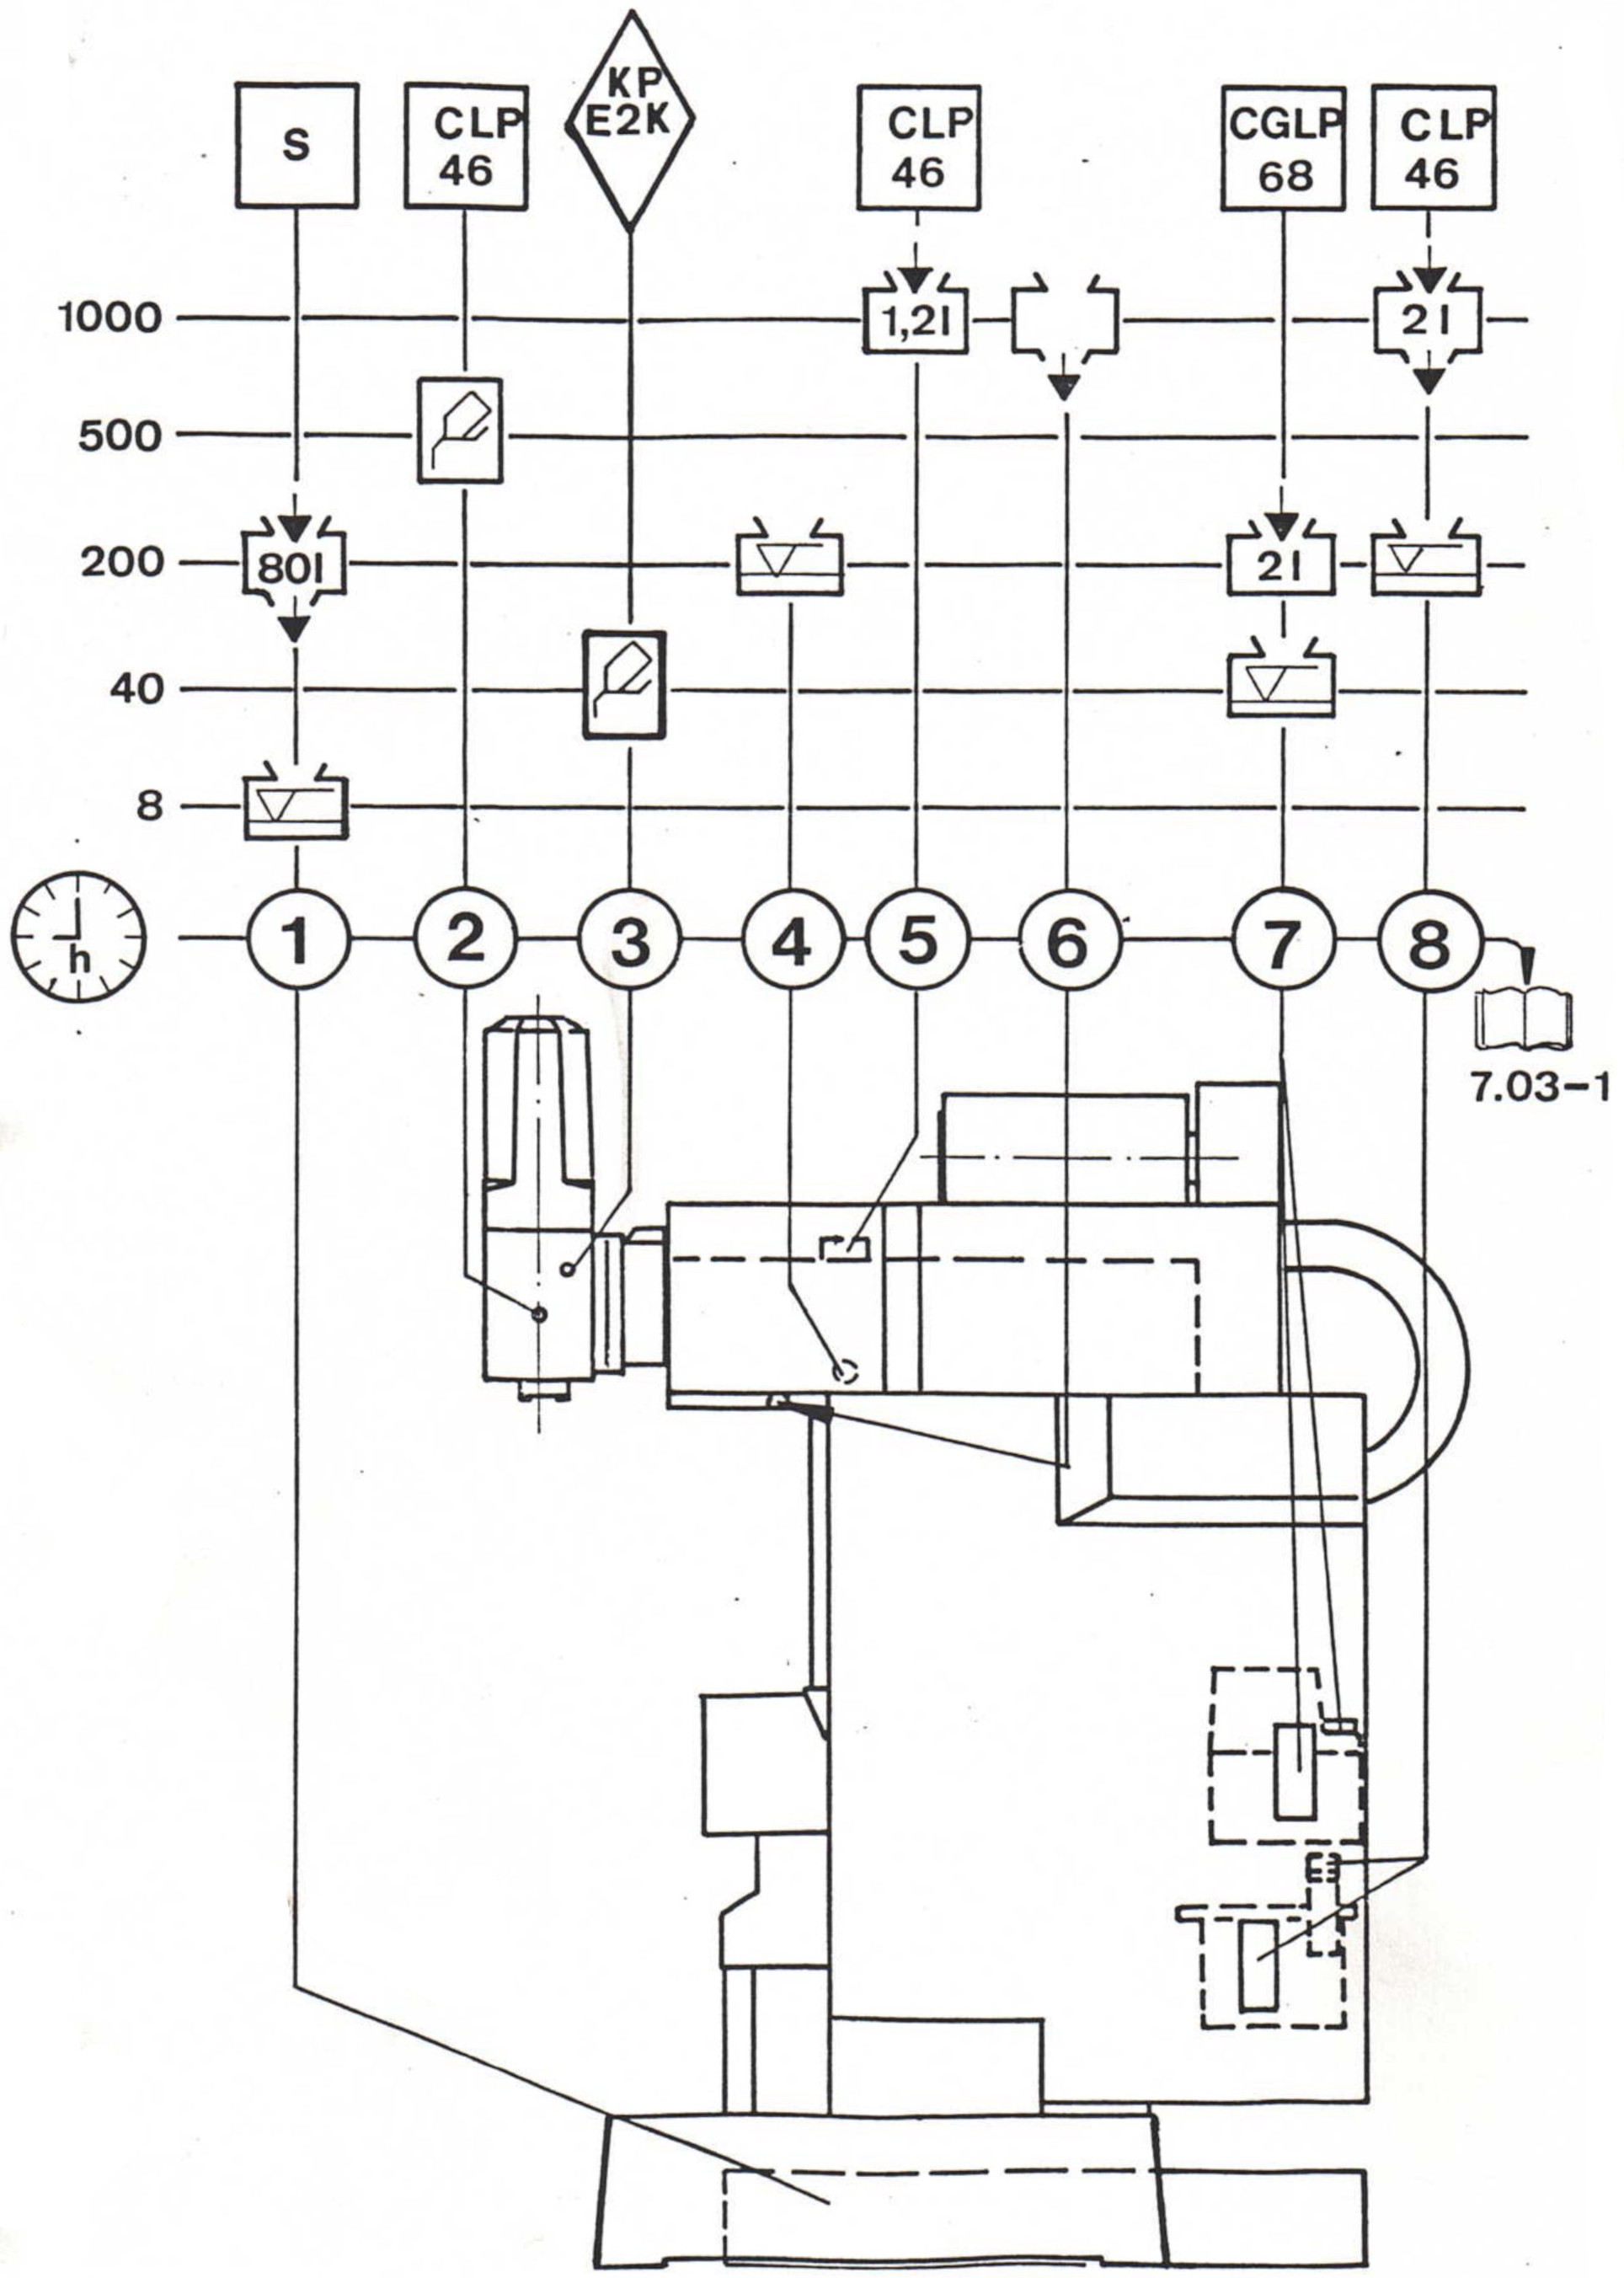
\includegraphics[width=0.9\textwidth]{chapter7/machine_lubrication_plan.jpg}
\end{figure}

\setsectiontitle{Lubrication Schedule}


\begin{table}[H]
    \centering
    \renewcommand{\arraystretch}{1.3}
    \begin{tabular}{|p{2cm}|p{1cm}|p{1.2cm}|p{7cm}|p{2cm}|p{2cm}|}
        \hline
        \hline
        \textbf{Interv. in Operating Hours} & \textbf{No. in Plan} & \textbf{Task Symbol} & \textbf{Task Description} & \textbf{Quantity} & \textbf{See Sheet} \\
        \hline
        \hline
        \multirow{1}{*}{8} & 1 & \raisebox{-\height}{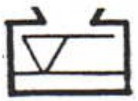
\includegraphics[width=10mm]{chapter7/coolant_level_check.jpg}} & Check coolant level in the coolant reservoir (keep as full as possible). & ---- & 3.22-1 \\
        \hline
        \multirow{2}{*}{40} & 3 \footnotemark[1] & \raisebox{-\height}{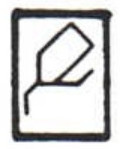
\includegraphics[width=10mm]{chapter7/lubrication.jpg}} & Lubricate bevel gear in the vertical milling head with Klüber-Isoflex NBU 15 (1 nipple, yellow marking). & 2-3 strokes & ---- \\
        \cline{2-6}
        & 7 & \raisebox{-\height}{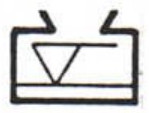
\includegraphics[width=10mm]{chapter7/oil_check.jpg}} & Check oil level in the central lubrication unit, refill if necessary. & ---- & 3.20-3 \\
        \hline
        \multirow{4}{*}{200} & 1 & \raisebox{-\height}{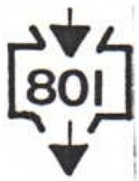
\includegraphics[width=10mm]{chapter7/coolant_change.jpg}} & Change coolant, clean tank. & approx. 80 l & 3.22-1, 7.07-4 \\
        \cline{2-6}
        & 4 & \raisebox{-\height}{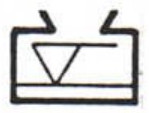
\includegraphics[width=10mm]{chapter7/oil_check.jpg}} & Check oil level for drive wheel, refill at position 5 if level drops below position 6. & ---- & ---- \\
        \cline{2-6}
        & 7 & \raisebox{-\height}{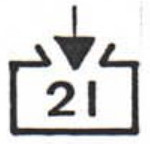
\includegraphics[width=10mm]{chapter7/oil_fill.jpg}} & Refill oil into the central lubrication unit. & max. 2 l & 3.20-3 \\
        \cline{2-6}
        & 8 & \raisebox{-\height}{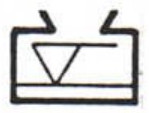
\includegraphics[width=10mm]{chapter7/oil_check.jpg}} & Check oil level in hydraulic unit. & ---- & 3.18-3 \\
        \hline
        \multirow{2}{*}{500} & 2 & \raisebox{-\height}{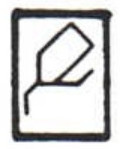
\includegraphics[width=10mm]{chapter7/lubrication.jpg}} & Lubricate quill in vertical milling head (1 nipple, red marking). & 2-3 strokes & ---- \\
        \hline
        \multirow{2}{*}{1000} & 5,6 & \raisebox{-\height}{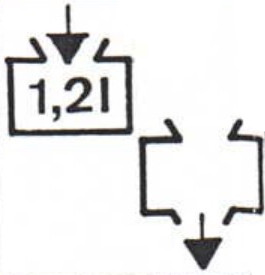
\includegraphics[width=13mm]{chapter7/oil_renew.jpg}} & Renew oil bath for drive wheel of horizontal spindle. & approx. 1,2 l & ---- \\
        \cline{2-6}
        & 8 & \raisebox{-\height}{
\includegraphics[width=10mm]{chapter7/oil_filter.jpg}} & Change hydraulic oil, clean filter. & max. 2 l & 3.18-3 \\
        \hline
        \hline
    \end{tabular}
\end{table}

\footnotetext[1]{For maximum load, e.g., continuous operation at maximum speed, lubricate every 8 operating hours!}

\setsectiontitle{Lubricant Recommendations}
\setcounter{section}{6}

\begin{table}[h]
    \centering
    \renewcommand{\arraystretch}{1.3}
    \begin{tabular}{|p{.75cm}|p{4cm}|p{2.7cm}|p{2.5cm}|p{4cm}|c|}
        \hline
        \hline
        \multicolumn{2}{|c|}{\textbf{Lubrication Point}} & \multicolumn{4}{c|}{\textbf{Lubricant Overview \footnotemark[1]}} \\
        \hline
        \hline
        \textbf{No. in Plan} & \textbf{Designation} & \textbf{Initial Fill Lubricant} & \textbf{Lubricant Type} & \textbf{Viscosity Range at 40°C / Analysis Data} & \textbf{Symbol} \\
        \hline
        \hline
        2 \newline 5 \newline 8 & Quill of the vertical milling head, Drive wheel of the horizontal work spindle, Hydraulic unit & Aral-Sumorol CM 46 (CMU) & Lubricating oil & CLP46/HLP46 41.4 - 50.6 & \raisebox{-\height}{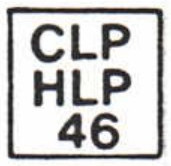
\includegraphics[height=8mm]{chapter7/clp_hlp_46.jpg}} \\
        \hline
        7 & Central lubrication unit, Universal built-in rotary table & Esso-Febis K 68 & Slideway oil & CGLP 68 (CG-HLP 68)/ 61.2 - 74.8 & \raisebox{-\height}{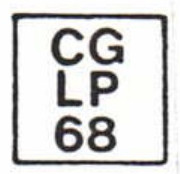
\includegraphics[height=8mm]{chapter7/cglp_68.jpg}} \\
        \hline
        3 & Bevel gear of the vertical milling head & Klüber-Iso-\newline flex \newline NBU 15 & Lubricating grease & KP E2K /\newline Walk penetration 265-295, Drip point approx. 180°C & \raisebox{-\height}{
\includegraphics[height=15mm]{chapter7/kp_e2k.jpg}} \\
        \hline
        1 & Cooling lubricant system & See Sheet 7.07-1 & Cooling lubricant & --- & \raisebox{-\height}{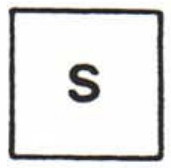
\includegraphics[height=8mm]{chapter7/s.jpg}} \\
        \hline
        \hline
    \end{tabular}
\end{table}

\footnotetext[1]{See Sheet 7.01-1 "Important Notes".}

\noindent Only the use of these lubricant types ensures the safe operation of the machine.  
We recommend continuing to use the initially filled lubricants, or if necessary, an equivalent type chosen based on operational requirements.

\notebox{WARNING}{\textbf{Liability cannot be accepted for the lubricants recommended in the following table.}}

Each of the lubricant manufacturers listed below maintains a lubrication service that can provide guidance and recommendations for all lubrication-related questions.

For intensive use of cooling lubricants, particularly in emulsion form the compatibility with the slideway oils used in the machine must be considered. See pages 7.07-1 to 7.07-3.

\newpage
\subsection{Lubricant Selection Table}

\textcolor{RoyalBlue}{\textbf{Initial fill lubricants}} are highlighted in blue to indicate the factory-recommended oils. These should be used whenever possible to ensure proper machine function and longevity.

\renewcommand{\arraystretch}{1.3}
\begin{longtable}{|p{2.2cm}|p{2.7cm}|p{3cm}|p{3cm}|p{4.5cm}|}
    \hline
    \multicolumn{1}{|c|}{} & 
    \multicolumn{4}{c|}{\textbf{Lubricant Identification According to DIN 51 502}} \\
    \hline
    \textbf{Oil Type / Manufacturer} & 
    \raisebox{-\height}{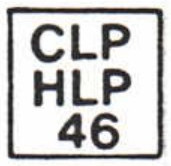
\includegraphics[height=15mm]{chapter7/clp_hlp_46.jpg}} & 
    \raisebox{-\height}{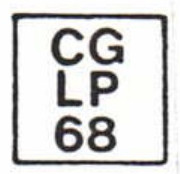
\includegraphics[height=15mm]{chapter7/cglp_68.jpg}} & 
    \raisebox{-\height}{
\includegraphics[height=15mm]{chapter7/kp_e2k.jpg}} & 
    \raisebox{-\height}{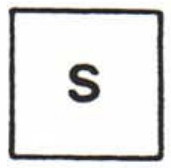
\includegraphics[height=15mm]{chapter7/s.jpg}} \newline \textbf{Cooling Lubricant} \\
    \hline
\endfirsthead

\hline
\multicolumn{1}{|c|}{} & 
\multicolumn{4}{c|}{\textbf{Lubricant Identification According to DIN 51 502}} \\
\hline
\textbf{Oil Type / Manufacturer} & 
\raisebox{-\height}{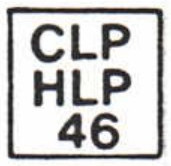
\includegraphics[height=15mm]{chapter7/clp_hlp_46.jpg}} & 
\raisebox{-\height}{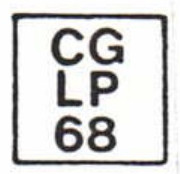
\includegraphics[height=15mm]{chapter7/cglp_68.jpg}} & 
\raisebox{-\height}{
\includegraphics[height=15mm]{chapter7/kp_e2k.jpg}} & 
\raisebox{-\height}{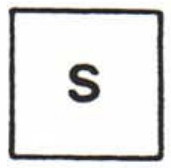
\includegraphics[height=15mm]{chapter7/s.jpg}} \newline \textbf{Cooling Lubricant} \\
\hline
\endhead
% Start of table body
    \hline
    ARAL & \textcolor{RoyalBlue}{\textbf{Sumorol CM 46}} & Aral-Deganit \newline BW 68 & --- & Sarol EP \newline Sarol 3965 \\
    \hline
    AVIA & AVILUB RL 46 \newline AVILUB HLPD 46 & AVILUB RSL 68-S & --- & AVILUB - Metacon ASBF \\
    \hline
    BP & Energol HL 46 \newline Energol HLP 46 & Maccurat 68 D & --- & (Cutora HX-Fedaro M) \\
    \hline
    Castrol & VARIO HDX \newline HYSPIN AWS 46 & MAGNA BDX 68 & --- & Clearedge EP 2840 \newline Hysol CB - Syntilo R \\
    \hline
    elf & POLYTELYS 46 \newline ELFOLNA 46 & MOGLIA 68 & --- & (Sarelf EP 34) \\
    \hline
    ESSO & NUTO H 46 \newline TERESSO 46 & \textcolor{RoyalBlue}{\textbf{FEBIS K 68}} & --- & Kutwell 30 \newline Kutwell 40 \\
    \hline
    FINA & FINA \newline HYDRAN CN 6 & ARTAC EP 68 & --- & (FINA VULSOL BST) \\
    \hline
    Fuchs & RENOLIN MR 15 & RENEP 2 & --- & RATAK DURANT 20 \newline RATAK TN 14/21 \\
    \hline
    Klüber & LAMORA 46 & LAMORA SUPER-POLADD 68 & \textcolor{RoyalBlue}{\textbf{Klüber Isoflex NBU 15}} & (ZELIOT-MS 250) \\
    \hline
    Mobil & D.T.E - Oil Medium \newline Mobil D.T.E 25 & BettbahnOil 68 & --- & Mobilmet 120 \newline Mobilmet 150 \newline EX 66/122 CF 1 \\
    \hline
    ÖMV & HTU 46 \newline HLP 46 & G 68 & --- & --- \\
    \hline
    Shell & Shell Tellus Oil C 46 \newline Shell Tellus Oil 46 & Tonna-Oil T 68 & --- & Shell-Dromus Oil BX \newline Shell-Dromus Oil EP \newline Shell-A 44 \\
    \hline
    TEXACO & Rando Oil 46 \newline HDB - 46 & Way Lubricant 68 & --- & Soluble Oil BS EP \newline Soluble Oil E \\
    \hline
    WISURA & Dynex 46 \newline Tempo 46 & BettbahnOil \newline 68 S (CGHLP 68) & --- & (Tralumat) \newline (WM 2998) \\
    \hline
    Zeller + Gmelin & GWA 2 ISO 46 \newline DHG 46 ISO & T 6 EP ISO 68 & --- & (Zubora 2000) \newline (Zubora 722 EP) \\
    \hline
\end{longtable}

\setsectiontitle{Coolants\protect\footnotemark[1]}
\setrevision{859}

For our milling machines and machining centers, only water-miscible and mineral-based coolant lubricants (in accordance with DIN 51385) should be used.

When selecting a coolant lubricant, care must be taken to ensure that the following undesirable properties \textbf{do not} occur:

\begin{enumerate}
    \item Adhesion and resinification of machine and control components, even if the coolant \\lubricant only enters in small quantities and cannot drain away.
    \item Incompatibility with the slideway oils used, which may cause them to decompose, harden, or be washed away.
    \item Corrosion protection must not decrease even after prolonged use of the coolant lubricant.
    \item Materials used in the machine for seals, wipers, etc. must not be attacked.
\end{enumerate}

\subsection*{Requirements for Coolant Lubricants\footnotemark[2]}

\begin{itemize}
    \item Good emulsifiability and stability even in harder water above 15° dH (5.4 m val).
    \item No damaging effects on machine components (metals, coatings, elastomers).
    \item Good lubricating properties and effectiveness for sliding machine elements.
    \item High resistance to decomposition and bacterial infestation.
    \item No harmful effects on humans.
    \item Toxicological test results and expert reports on skin compatibility should be available.
    \item No toxic additives such as nitrites or phenols.
    \item Must at least comply with the technical regulations for hazardous substances (TRgA 900).
    \item Used coolant lubricant emulsions must be separable by conventional separation processes.
\end{itemize}

\footnotetext[1]{DIN 51 385: 
\begin{minipage}[t]{\textwidth}
    \begin{itemize}
        \item Term 2.1 = Emulsifiable coolant lubricant (concentrate)
        \item Term 3.1 = Coolant lubricant emulsion (oil-in-water), ready-to-use mixture.
    \end{itemize}
    \vspace{.1cm}
\end{minipage}
}
\footnotetext[2]{See data sheet 7.07-2, 7.07-2.1.}
\newpage

\subsection{Data Sheet}

Selection criteria based on VKIS-Worksheet 3 - Sept. 83.

\subsubsection*{Physical and Chemical Reference Values}

\subsubsection*{6.1 Coolant Lubricant Concentrate}

\renewcommand{\arraystretch}{1.3}
\begin{longtable}{|p{6cm}|p{3cm}|p{3.5cm}|p{3.5cm}|}
    \hline
    \textbf{Property} & \textbf{Unit} & \textbf{Test Method} & \textbf{Reference Values} \\
    \hline
    \endfirsthead

    \hline
    \textbf{Property} & \textbf{Unit} & \textbf{Test Method} & \textbf{Reference Values} \\
    \hline
    \endhead

    \hline
    \endfoot

    \hline
    \endlastfoot

    Total mineral oil content & Vol. \% & DIN 51 417E & $> 35$ \\
    \hline
    Water content & Vol. \% & DIN 51 582 & Must be specified \\
    \hline
    Density & g/cm³ at 20°C & DIN 51 757 & 0.93 - 1.06 \\
    \hline
    Kinematic viscosity at 40°C & mm²/s (cSt) & DIN 51 366 & 20 - 120 \\
    \hline
    Kinematic viscosity at 20°C & mm²/s (cSt) & DIN 51 562 \newline DIN 53 015 & 50 - 300 \\
    \hline
    Refractive index & $n_D$ 20°C & DIN 51 423 & Must be specified \\
    \hline
    Flash point & + °C & DIN 51 376 & $> 130$ \\
    \hline
    Pour point & - °C & DIN 51 583 & 10 - 15 \\
    \hline
    EP additives (Mass. \%) & P \newline S \newline CI & DIN 51 363 \newline DIN 51 400 \newline DIN 51 577 & Must be specified \\
    \hline
    Sulfated ash (Mass. \%) &  & DIN 51 575 & --- \\
    \hline
    Preservatives & --- & --- & Type and amount must be specified \\
    \hline
    Silicones & \% & --- & Must be specified \\
    \hline
    Boron content & --- & --- & Must be specified \\
    \hline
    IR Spectrum & --- & --- & Must be specified \\
    \hline
\end{longtable}

\subsubsection*{6.2 Water-Mixed Coolant Lubricant (Emulsion)}

\renewcommand{\arraystretch}{1.3}
\begin{longtable}{|p{6cm}|p{3cm}|p{2cm}|p{2.5cm}|p{2cm}|}
    \hline
    \textbf{Property} & \textbf{Concentration} & \textbf{Unit} & \textbf{Test Method} & \textbf{Reference} \newline \textbf{Values} \\
    \hline
    \endfirsthead

    \hline
    \textbf{Property} & \textbf{Concentration} & \textbf{Unit} & \textbf{Test Method} & \textbf{Reference} \newline \textbf{Values} \\
    \hline
    \endhead

    \hline
    \endfoot

    \hline
    \endlastfoot

    pH value at:\footnotemark[1] \newline NW12 (12°d.H.)\footnotemark[2] & 
    2\% \newline 10\% & 
    --- & 
    DIN 51 369 & 
    8 - 9.4 \\
    \hline
    Thermal conductivity & 5\% & kcal/mh°C & --- & $> 0.45$ \\
    \hline
\end{longtable}

\footnotetext[1]{\hangindent=1.8em The pH value is a measure of alkalinity. A pH of 7.0 is neutral (e.g., pure drinking water). Emulsions with a pH lower than 7.0 are considered \enquote{acidic} and provide poor corrosion protection. Higher pH values (up to 10.0) improve corrosion resistance. However, a pH greater than 9.4 can cause etching on sliding machine elements and skin irritation for operators.}
\footnotetext[2]{%
\hangindent=1.8em "NW12" refers to \enquote{normal water} with a hardness of 12° d.H. (4.3 mval.).  
\\ 100 d.H. means: 10g calcium oxide per 100 liters of water.  
\enquote{d.H.} is the abbreviation for \enquote{Deutsche Härte} (German hardness), for example:  

\begin{description}
    \item[\hspace{1.8em}Soft water:] less than 6° d.H. \footnotemark[5]
    \item[\hspace{1.8em}Moderately hard water:] 6 - 12° d.H.
    \item[\hspace{1.8em}Hard water:] more than 12° d.H.
\end{description}

\hspace{.3em} The hardness of tap water can be obtained from the local water utility.
}

\newpage

\subsubsection*{Additional Physicochemical Reference Values}
\setcounter{page}{2}
\setsubpage{1}
Selection criteria based on VKIS-Worksheet 3 - Sept. 83.

\renewcommand{\arraystretch}{1.3}
\begin{longtable}{|p{5cm}|p{1.5cm}|p{3.5cm}|p{3cm}|p{2.5cm}|}
    \hline
    \textbf{Property} & \textbf{Concen-} \newline \textbf{tration} & \textbf{Unit} & \textbf{Test Method} & \textbf{Reference Values} \\
    \hline
    \endfirsthead

    \hline
    \textbf{Property} & \textbf{Concen-} \newline \textbf{tration} & \textbf{Unit} & \textbf{Test Method} & \textbf{Reference Values} \\
    \hline
    \endhead

    Electrical conductivity & 5\% & $\mu$S/cm & DIN 38 404 & Must be specified \\
    \hline
    Corrosion protection capacity & 5\% & --- & DIN 51 360/1 & RO, SO\footnotemark[3] \\
    \hline
    Corrosion degree & 5\% & --- & DIN 51 360/2 & 0 \\
    \hline
    Corrosion effect on copper\footnotemark[4] & 2.5\% & mg/dm³ & VKIS-Worksheet No. 7 \newline (DIN 51 759) & --- \\
    \hline
    Stability \newline (with 3g NaCl/1) & 5\% & --- & DIN 51 367 & $<$ 95\% \\
    \hline
    Foam behavior at NW 12 & 5\% & --- & --- & To be agreed upon with the manufacturer \\
    \hline
    Adhesion and residue behavior & 5\% & --- & VKIS-Worksheet No. 9 & Non-sticky, slightly soluble \\
    \hline
    Behavior against elastomers S2 according to DIN 53504\footnotemark[4] & --- & --- & --- & See Table~\ref{tab:elastomer_test} \\
    \hline
    Acid-decomposable components & 2\% \newline 10\% & Mass. \% & DIN 51 368 & Must be specified \\
    \hline
    EP-Effect & --- & --- & VKIS-Worksheet No. 6 & --- \\
    \hline
    Wear resistance according to Reichert & 5\% & N/cm² & --- & Must be specified \\
    \hline
\end{longtable}

\renewcommand{\arraystretch}{1.3}
\begin{longtable}{|p{5cm}|p{1.5cm}|p{5.5cm}|p{4cm}|}
    \caption{Elastomer Test Results} \label{tab:elastomer_test} \\
    \hline
    \textbf{Elastomer Material} & \textbf{Concen-} \newline \textbf{tration} & \textbf{Test Method} & \textbf{Result} \\
    \hline
    \endfirsthead

    \hline
    \textbf{Elastomer Material} & \textbf{Concen-} \newline \textbf{tration} & \textbf{Test Method} & \textbf{Result} \\
    \hline
    \endhead

    \hline
    \endfoot

    \hline
    \endlastfoot

    \multirow{2}{*}{SRE-WBR 28} & 2\% & VDA-Prüfblatt 521-01 \newline (DIN E 53 538) & +0.5\% Vol. Change \\
    & 10\% & --- & +0.15\% Shore-A Change \\
    \hline
    \multirow{2}{*}{CFW 88 NBR/101} & 2\% & --- & --- \\
    & 10\% & --- & --- \\
    \hline
\end{longtable}

\footnotetext[3]{RO = No rust; SO = No black spotting.}
\footnotetext[4]{Discoloration: None, Deposit formation: None, Copper ion content: Max. 50.}
\footnotetext[5]{\hangindent=1.8em International notation for water hardness is "mval." (Sum of all dissolved minerals). Conversion: $\frac{\text{dH}}{2.8}$}

\newpage
\subsection{Coolant Lubricant Recommendations}
\clearsubpage
\setrevision{7631}
(July '86)

The following coolant lubricants (\textbf{except those marked in \textcolor{RoyalBlue}{RoyalBlue}}) have been tested in the lab, evaluated positively according to the \textbf{DIN 51 599 standard} for demulsification using the stir test method.

Since the exact \textbf{application conditions} are beyond our knowledge and control, we\\ \textbf{cannot guarantee} the suitability of these products.

\notebox{WARNING}{%
    \textbf{LEGAL LIABILITY CANNOT BE DERIVED FROM THIS RECOMMENDATION LIST!}
}

If, for \textbf{production-related reasons}, lubricants \textbf{other than} those listed here must be used, they must comply with the \textbf{selection criteria} outlined in sheets \textbf{7.07-2 to 7.07-2.2}.

\renewcommand{\arraystretch}{1.3}
\begin{longtable}{|p{3.5cm}|p{4.5cm}|p{1.5cm}|p{2.7cm}|p{2cm}|}
    \caption{Coolant Lubricant Recommendations (July '86)}
    \label{tab:coolant_lubricants} \\
    \hline
    \textbf{Manufacturer} & \textbf{Product Name} & \textbf{Mineral Oil \%} & \textbf{Mix Ratio} & \textbf{Concentr-} \newline \textbf{ation(\%)} \\
    \hline
    \endfirsthead

    \hline
    \textbf{Manufacturer} & \textbf{Product Name} & \textbf{Mineral Oil \%} & \textbf{Mix Ratio} & \textbf{Concentr-} \newline \textbf{ation(\%)} \\
    \hline
    \endhead

    \hline
    \endfoot

    \hline
    \endlastfoot

    \multirow{2}{*}{ACMOS} & ACMOSIT 64-02 & 30 & 1:20 - 1:30 & 5 - 3 \\
    \cline{2-5}
    & \textcolor{RoyalBlue}{Emulsol 230} & 72 & 1:20 - 1:50 & 5 - 2 \\
    \hline

    \multirow{2}{*}{Aral} & \textcolor{RoyalBlue}{Sarol EP} & 37 & 1:10 - 1:30 & 10 - 3 \\
    \cline{2-5}
    & Sarol 3965 & 25 & 1:10 - 1:50 & 10 - 2 \\
    \hline

    \multirow{2}{*}{AVIA (Bantleon)} & \textcolor{RoyalBlue}{AVILUB - HSK-EP} & 50 & 1:10 - 1:40 & 10 - 2.5 \\
    \cline{2-5}
    & AVILUB - Metacon ASBF & 35 & 1:20 - 1:50 & 5 - 2 \\
    \hline

    \multirow{2}{*}{Belluco \& Co.} & Sintolin E1/MH & 70 & 1:20 - 1:30 & 5 - 3 \\
    \cline{2-5}
    & Sintolin CB 1/MH & --- & 1:20 - 1:30 & 5 - 3 \\
    \hline

    \multirow{2}{*}{BP} & Olex SB 5580 CF & 40 & 1:20 - 1:40 & 5 - 2.5 \\
    \cline{2-5}
    & Fedaro M & 75 & 1:5 - 1:30 & 20 - 3 \\
    \hline

    \multirow{2}{*}{Blaser} & Blascout 2000 Univ. & 62 & 1:3 - 1:20 & 33 - 5 \\
    \cline{2-5}
    & \textcolor{RoyalBlue}{Blascout 4000 Strong} & 43 & 1:3 - 1:20 & 33 - 5 \\
    \hline

    \multirow{3}{*}{Castrol} & Clearedge EP 2840 & 42 & 1:20 - 1:30 & 5 - 3 \\
    \cline{2-5}
    & Hysol CB & 48 & 1:25 - 1:50 & 4 - 2 \\
    \cline{2-5}
    & Syntilo R (TLS 984 in USA) & 40 & 1:20 - 1:40 & 5 - 2.5 \\
    \hline

    \multirow{1}{*}{Chemie Linz AG} & Hardcoor S 305 & --- & --- & --- \\
    \hline

    \multirow{2}{*}{\shortstack[l]{Cincinnati-\\Milacron}} & Cimperial 22 & 56 & 1:10 - 1:30 & 10 - 3 \\
    \cline{2-5}
    & Cimcool MB 602 & 37 & 1:10 - 1:40 & 10 - 2.5 \\
    \hline

    \multirow{2}{*}{CMT - Raunheim} & Aquasol 6-58 & 52 & 1:20 - 1:40 & --- \\
    \cline{2-5}
    & \textcolor{RoyalBlue}{Universal 6-58} & 36 & 1:10 - 1:30 & --- \\
    \hline

    \multirow{2}{*}{Consulta-Chemie} & Rondocor Kompakt & 44 & 1:20 - 1:50 & 5 - 2 \\
    \cline{2-5}
    & Rondocor 6459 & --- & --- & --- \\
    \hline

    \multirow{3}{*}{Curtis} & S-6 & 53 & 1:5 - 1:20 & 20 - 5 \\
    \cline{2-5}
    & S-12 & --- & 1:1 & --- \\
    \cline{2-5}
    & S-21 & 25 & 1:10 - 1:20 & 10 - 5 \\
    \hline

    \multirow{1}{*}{elf} & \textcolor{RoyalBlue}{Sarelf E P34} & 30 & 1:20 - 1:50 & 5 - 2 \\
    \hline

    \multirow{2}{*}{ESSO} & Bohroel BS 30 & --- & --- & --- \\
    \cline{2-5}
    & \textcolor{RoyalBlue}{Kutwell 40} & 83 & 1:10 - 1:40 & 10 - 2.5 \\
    \hline

    \multirow{1}{*}{FINA} & \textcolor{RoyalBlue}{VULSOL BST} & 40 & 1:20 - 1:50 & 5 - 2 \\
    \hline
\end{longtable}

\newpage
\setcounter{page}{3}
\setsubpage{1}

\renewcommand{\arraystretch}{1.3}
\begin{longtable}{|p{3.5cm}|p{4.5cm}|p{1.5cm}|p{2.7cm}|p{2cm}|}
    \caption{}
    \label{tab:coolant_lubricants_2} \\
    \hline
    \textbf{Manufacturer} & \textbf{Product Name} & \textbf{Mineral Oil \%} & \textbf{Mix Ratio} & \textbf{Concentr-} \newline \textbf{ation(\%)} \\
    \hline
    \endfirsthead

    \hline
    \textbf{Manufacturer} & \textbf{Product Name} & \textbf{Mineral Oil \%} & \textbf{Mix Ratio} & \textbf{Concentr-} \newline \textbf{ation(\%)} \\
    \hline
    \endhead

    \hline
    \endfoot

    \hline
    \endlastfoot

    \multirow{3}{*}{Fuchs} & RATAK DURANT 20 & --- & 1:10 - 1:40 & 10 - 2.5 \\
    \cline{2-5}
    & RATAK RESIST 31 & --- & 1:10 - 1:40 & 10 - 2.5 \\
    \cline{2-5}
    & RATAK TN 14/21 & 45 & 1:10 - 1:30 & 10 - 3 \\
    \hline

    \multirow{1}{*}{Henkel} & \textcolor{RoyalBlue}{P3-Multan 92-9} & 35 & 1:7 - 1:20 & 14 - 5 \\
    \hline

    \multirow{2}{*}{Houghton Chemie} & \textcolor{RoyalBlue}{ISCOUT 100} & ca. 50 & 1:10 - 1:40 & 10 - 2.5 \\
    \cline{2-5}
    & \textcolor{RoyalBlue}{ISCOUT Spezial} & ca. 45 & 1:20 & 5 \\
    \hline

    \multirow{2}{*}{Jokisch} & W2 OP & 32 & 1:7 - 1:20 & 14 - 5 \\
    \cline{2-5}
    & Kompakt W3 CF & 39 & 1:10 - 1:20 & 10 - 5 \\
    \hline

    \multirow{1}{*}{\shortstack[l]{Klüber \\Lubrication}} & \textcolor{RoyalBlue}{ZELIOT MS 250} & 20 & 1:5 - 1:20 & 20 - 5 \\
    \hline

    \multirow{4}{*}{Kocher} & Kocher - F 14 & 55 & 1:20 - 1:30 & 5 - 3 \\
    \cline{2-5}
    & Kocher - F 17 & 48 & 1:20 - 1:30 & 5 - 3 \\
    \cline{2-5}
    & Kocher - F100 & 60 & 1:20 - 1:30 & 5 - 3 \\
    \cline{2-5}
    & Kocher - PKT 5 & 56 & 1:10 - 1:30 & 10 - 3 \\
    \hline
    \multirow{2}{*}{\shortstack[l]{Lionoil (Master \\Chemical Corp.)}} & TRIM SOL & 45 & 1:10 - 1:30 & 10 - 3 \\
    \cline{2-5}
    & \textcolor{RoyalBlue}{Trim SOL Silicone Free} & 45 & 1:10 - 1:30 & 10 - 3 \\
    \hline

    \multirow{2}{*}{Lubricor} & M 735 & 50 & 1:10 - 1:20 & 10 - 5 \\
    \cline{2-5}
    & \textcolor{RoyalBlue}{B 421} & 20 & 1:20 - 1:30 & 5 - 3 \\
    \hline

    \multirow{4}{*}{Mobil} & Mobilmet 120 & 30 & 1:10 - 1:50 & 10 - 2 \\
    \cline{2-5}
    & Mobilmet 150 & 33 & 1:10 - 1:20 & 10 - 5 \\
    \cline{2-5}
    & Mobil EXD 16/122 CF & --- & 1:1 & --- \\
    \cline{2-5}
    & Mobilmet 220 & 25 & 1:20 - 1:30 & 5 - 3 \\
    \hline

    \multirow{1}{*}{MKU} & Betronol EPV 1530 & 54 & 1:15 - 1:30 & 7 - 3 \\
    \hline

    \multirow{3}{*}{Oemeta} & HD 52 & 30 & 1:10 - 1:30 & 10 - 3 \\
    \cline{2-5}
    & KR 586 & 60 & 1:10 - 1:30 & 10 - 3 \\
    \cline{2-5}
    & UNIMET SG 4 & 41 & 1:10 - 1:40 & 10 - 2.5 \\
    \hline

    \multirow{1}{*}{Optimol} & \textcolor{RoyalBlue}{CUTO W 200} & 78 & 1:10 - 1:30 & 10 - 3 \\
    \hline

    \multirow{3}{*}{Petrat} & \textcolor{RoyalBlue}{PRIMOL chlorfrei BKA/1} & 70 & 1:10 - 1:30 & 10 - 3 \\
    \cline{2-5}
    & \textcolor{RoyalBlue}{PRIMOL chlorfrei BK/84} & 60 & 1:10 - 1:30 & 10 - 3 \\
    \cline{2-5}
    & \textcolor{RoyalBlue}{PRIMOL chlorfrei BK/601 EP} & 60 & 1:10 - 1:25 & 10 - 4 \\
    \hline

    \multirow{3}{*}{Shell} & Shell-Dromus Oel BX & 80 & 1:10 - 1:20 & 10 - 5 \\
    \cline{2-5}
    & Shell-Dromus Oel EP & 45 & 1:12 - 1:20 & 8 - 5 \\
    \cline{2-5}
    & Shell-Dromus Oel D & 35 & 1:12 - 1:30 & 8 - 3 \\
    \hline

    \multirow{3}{*}{Texaco} & Soluble Oil BS EP & ca. 40 & 1:10 - 1:30 & 10 - 3 \\
    \cline{2-5}
    & Soluble Oil E & ca. 65 & 1:10 - 1:30 & 10 - 3 \\
    \cline{2-5}
    & Soluble Oil HDE & ca. --- & 1:1 & --- \\
    \hline
    \multirow{3}{*}{WISURA} & Tralumat & ca. 52 & 1:20 - 1:30 & 5 - 3 \\
    \cline{2-5}
    & \textcolor{RoyalBlue}{Tralustar} & ca. 44 & 1:10 - 1:20 & 10 - 5 \\
    \cline{2-5}
    & WM 2998 & ca. 40 & 1:20 - 1:30 & 5 - 3 \\
    \hline
\end{longtable}

\newpage
\setcounter{page}{3}
\setsubpage{2}

\renewcommand{\arraystretch}{1.3}
\begin{longtable}{|p{3.5cm}|p{4.5cm}|p{1.5cm}|p{2.7cm}|p{2cm}|}
    \caption{}
    \label{tab:coolant_lubricants_3} \\
    \hline
    \textbf{Manufacturer} & \textbf{Product Name} & \textbf{Mineral Oil \%} & \textbf{Mix Ratio} & \textbf{Concentr-} \newline \textbf{ation(\%)} \\
    \hline
    \endfirsthead

    \hline
    \textbf{Manufacturer} & \textbf{Product Name} & \textbf{Mineral Oil \%} & \textbf{Mix Ratio} & \textbf{Concentr-} \newline \textbf{ation(\%)} \\
    \hline
    \endhead

    \hline
    \endfoot

    \hline
    \endlastfoot

    \multirow{3}{*}{Zeller + Gmelin} & \textcolor{RoyalBlue}{Zubora 2000 EP} & ca. 58 & 1:10 - 1:40 & 10 - 2.5 \\
    \cline{2-5}
    & \textcolor{RoyalBlue}{Zubora 722 EP} & ca. 33.5 & 1:10 - 1:30 & 10 - 3 \\
    \cline{2-5}
    & \textcolor{RoyalBlue}{Zubora SM} & ca. 73 & 1:10 - 1:30 & 10 - 3 \\
    \hline
\end{longtable}

\newpage
\clearsubpage
\subsection*{Application Instructions for Water-Miscible Coolant Lubricants}
\setrevision{5523}
\subsubsection*{Initial Filling}
\begin{itemize}
    \item Completely remove the previous coolant lubricant from the system.
    \item Clean the container and machine from chips, sludge, and deposits.
    \item Flush with hot soda water (2 kg per 50 L of water).
    \item Remove soda water and rinse with clean tap water.
    \item Use system cleaner only for heavily contaminated systems.
\end{itemize}

\subsubsection*{Mixing}
\begin{itemize}
    \item Fill clean tap water into a clean container and add the appropriate amount of concentrate in a \textbf{thin stream} while stirring continuously.  
          \textbf{Never the other way around!}
    \item Do not use softened water. Ideal water hardness: \textbf{7 - 20° dH}.
    \item Do not store the emulsion in galvanized containers. Never mix prepared emulsion with other brands.
    \item Mixing temperature:  
          \quad Concentrate: \textbf{Min. +10°C}  
          \quad Water: \textbf{Max. +30°C}
    \item Only use pre-mixed emulsion in the container!
\end{itemize}

\subsubsection*{Monitoring}
\begin{itemize}
    \item Periodically check concentration using a \textbf{hand refractometer} or acid separation.  
          \\Refractometer reading factor: \textbf{1.0}
    \item If the concentration is too high, dilute with a \textbf{very lean emulsion/solution}  
          (\textbf{never add pure water!})
    \item Measure pH value using indicator paper or electrometrically.  
          Target range: \textbf{pH 8.3 - 9.0}.
    \item Continuously or periodically remove floating leakage oil.
    \item Contaminated emulsion can be filtered or decanted and reused.
    \item In case of \textbf{heavy contamination} (depending on bacterial resistance), replace coolant lubricant and clean the system.
    \item \textbf{Additives} such as \textbf{bactericides, rust inhibitors, and anti-foam agents} must \textbf{not} be used.
\end{itemize}

\setsectiontitle{Removing the Machine Covers}
\setrevision{7631}
\setcounter{section}{10}

\begin{figure}[H]
    \centering
    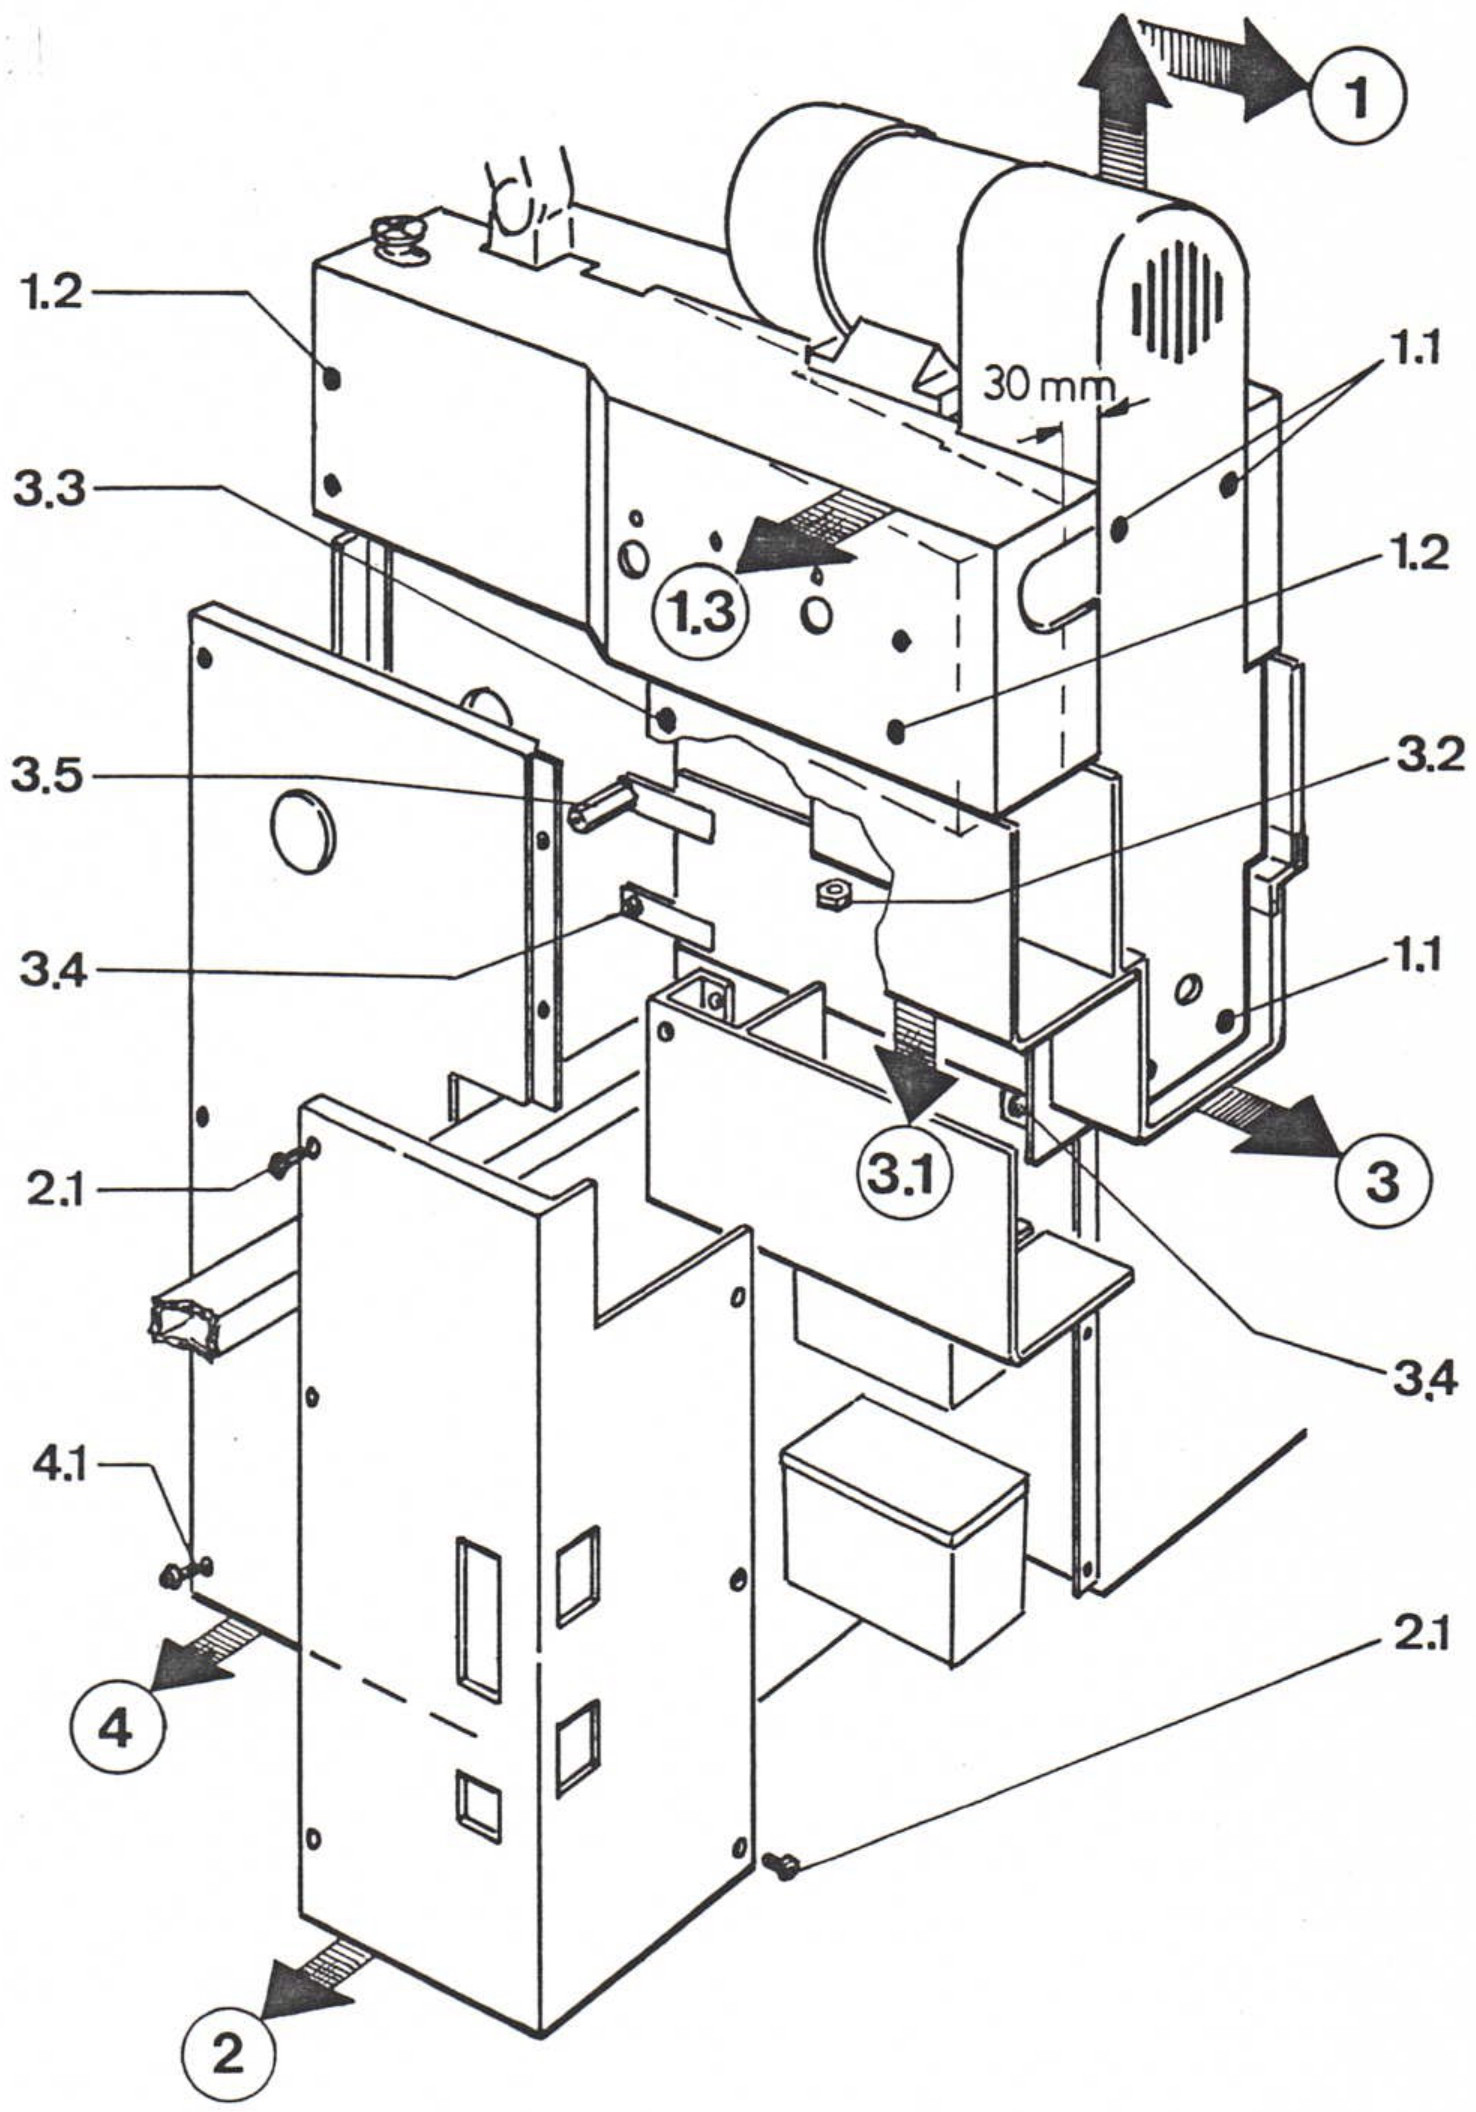
\includegraphics[width=0.7\textwidth]{images/chapter7/machine_cover_removal_diagram.jpg}
    \label{fig:machine_cover_removal}
\end{figure}

To perform \textbf{maintenance and adjustment work}, it is sometimes necessary to remove the \textbf{machine covers}.  
This is done for \circled{1}, \circled{2}, and \circled{4} after unscrewing the screws (\ellipsed{1.1} - \ellipsed{2.1} and \ellipsed{4.1}).

\notebox{WARNING}{%
    Before removing \circled{1}, loosen screws (\ellipsed{1.2}), and \textbf{push the hood (\ellipsed{1.3}) back about 30 mm}!  
    Before removing \circled{3}, remove \textbf{guide plate (\ellipsed{3.1})}.  
    To do this, unscrew \textbf{nuts (\ellipsed{3.2})}, \textbf{screws (\ellipsed{3.3})}, and \textbf{stud bolts (\ellipsed{3.5})}.
}

\setsectiontitle{Maintenance Plan}
\setrevision{5628}

\setcounter{section}{20}

See pages 7.21-1 and 7.22-1 \enquote{Overview of Maintenance Tasks}.

\begin{figure}[H]
    \centering
    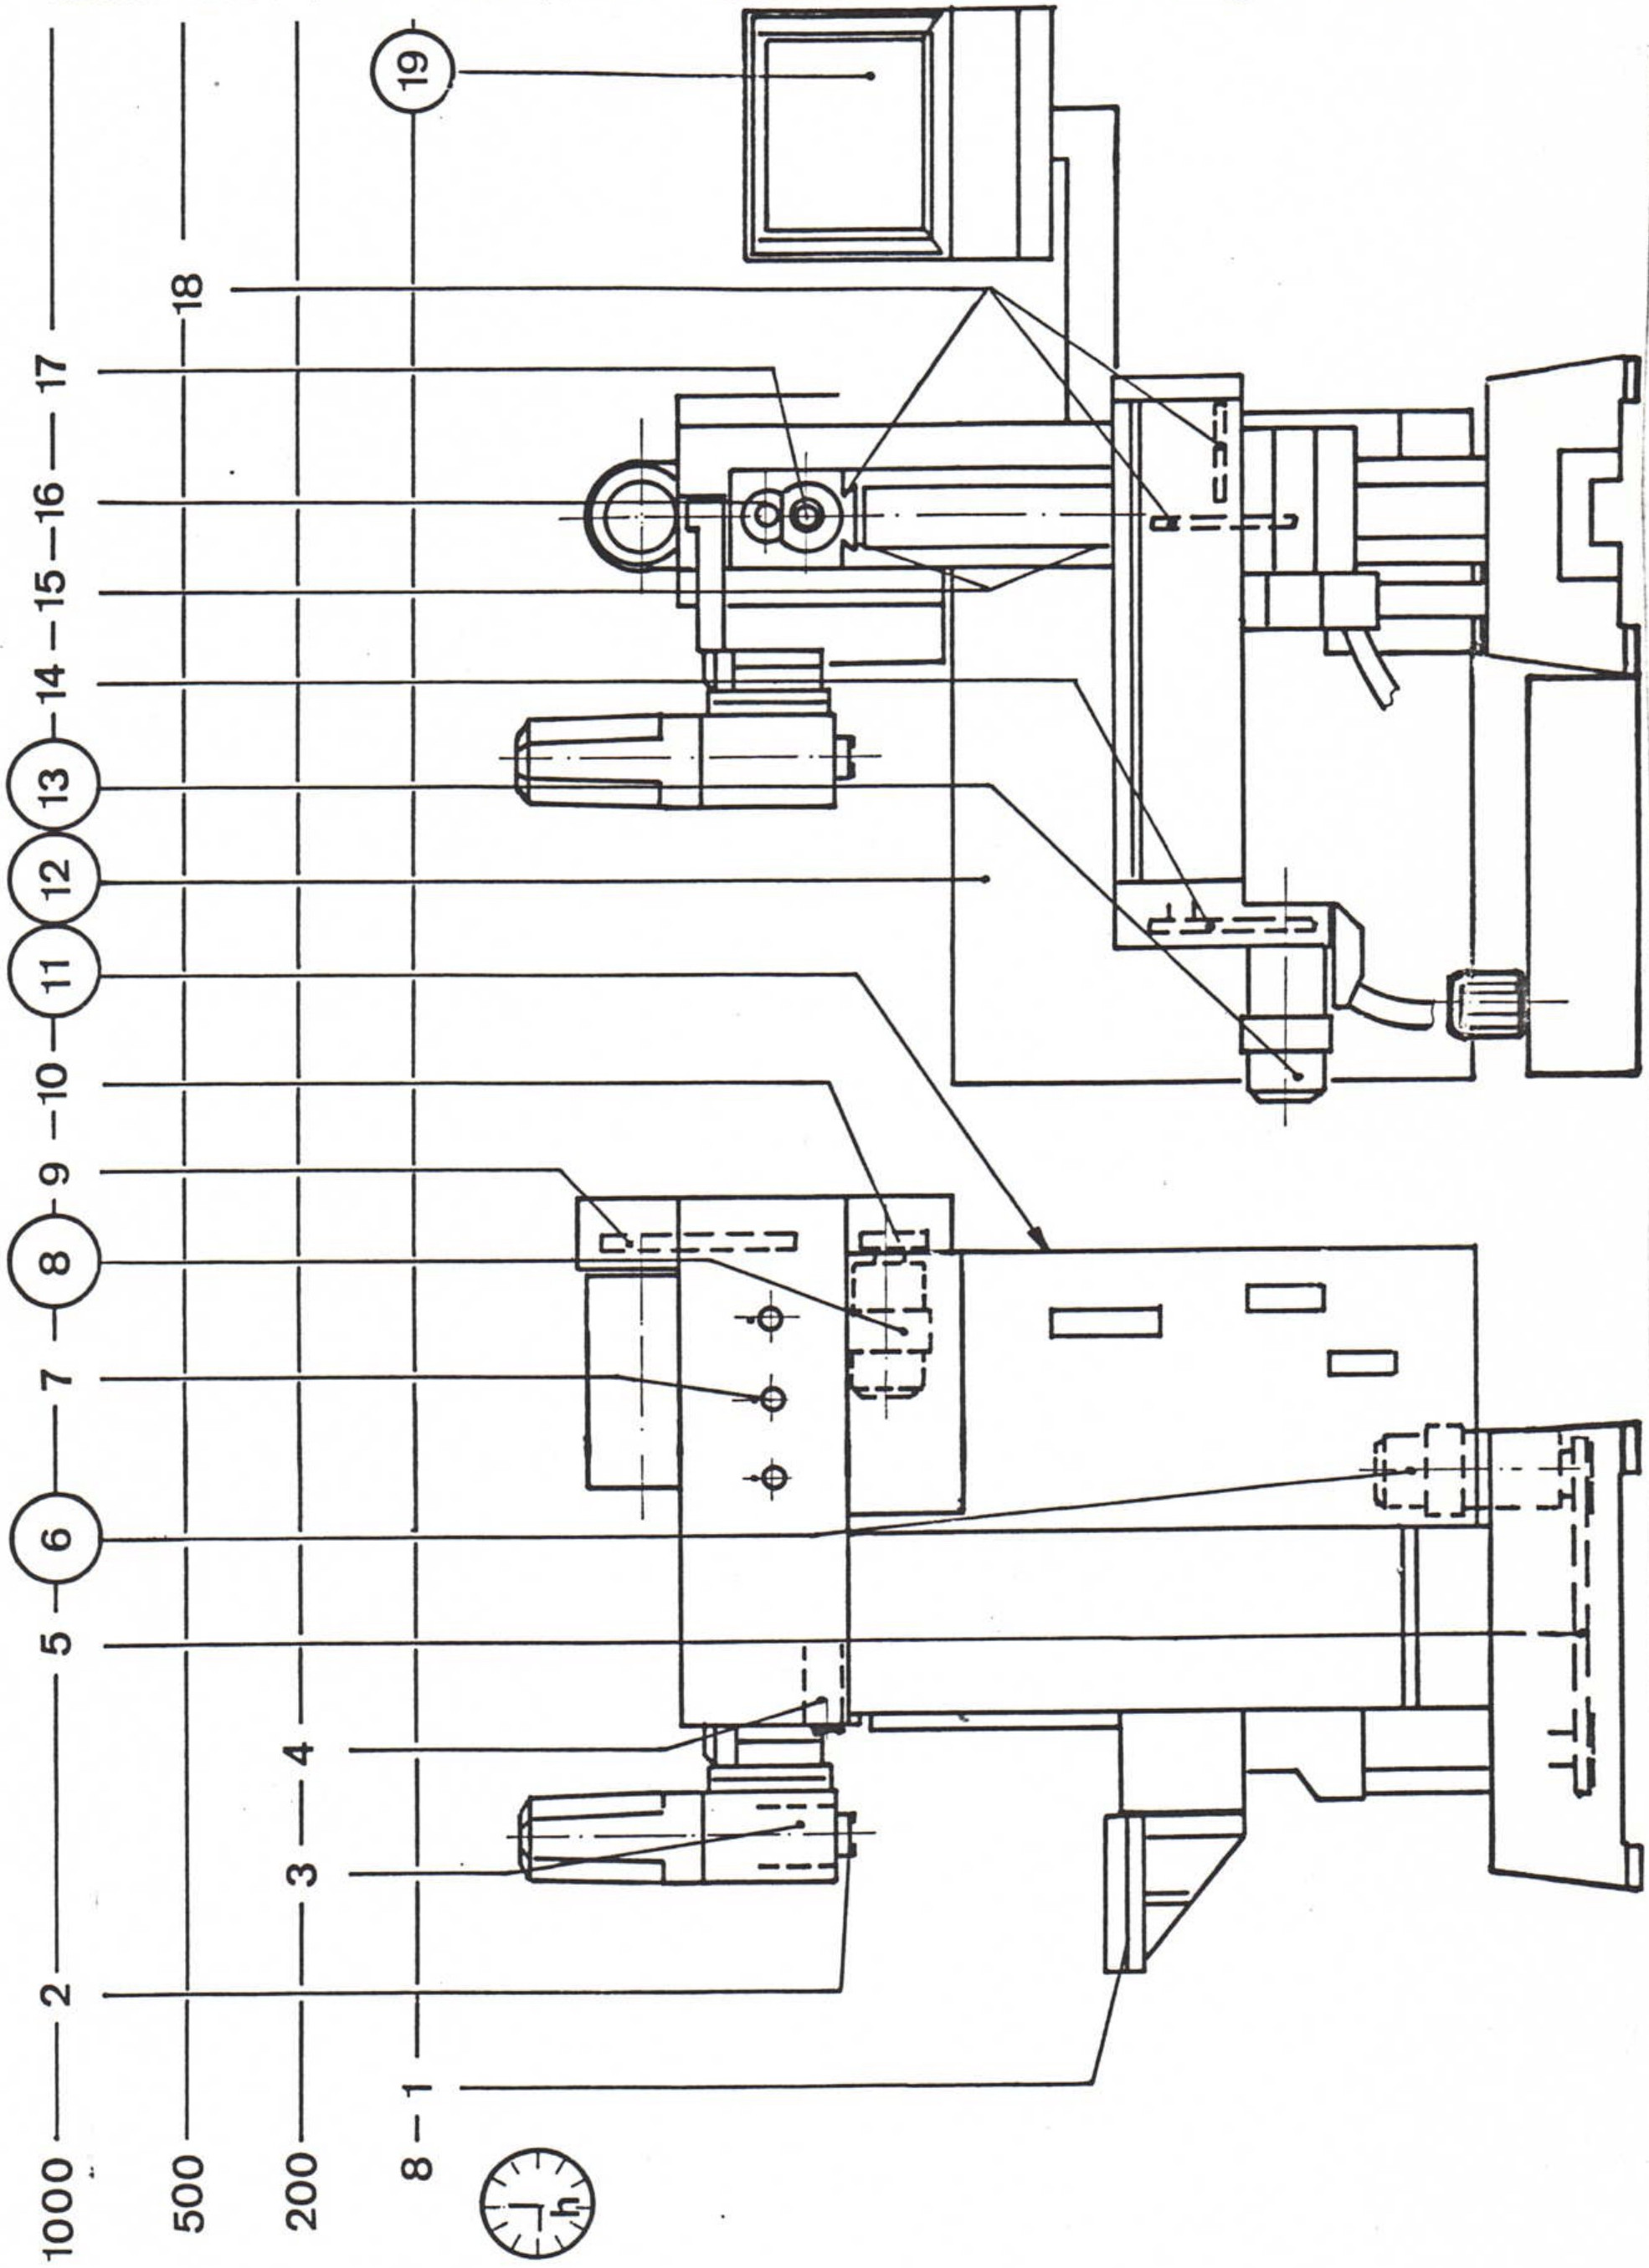
\includegraphics[width=0.9\textwidth]{images/chapter7/maintenance_plan_diagram.jpg}
    \label{fig:maintenance_plan}
\end{figure}

\setsectiontitle{Mechanics and Hydraulics Maintenance Tasks}
\setrevision{7631}

\renewcommand{\arraystretch}{1.3}
\begin{longtable}{|p{1.8cm}|p{1.2cm}|p{8.5cm}|p{2cm}|}
    \hline
    \textbf{Interval (Hrs)} & \textbf{Nr. in \newline plan} & \textbf{Task} & \textbf{See Sheet} \\
    \hline
    \endfirsthead

    \hline
    \textbf{Interval (Hrs)} & \textbf{Nr. in \newline plan} & \textbf{Task} & \textbf{See Sheet} \\
    \hline
    \endhead

    \hline
    \endfoot

    \multirow{1}{*}{8} & 1 & Clean the coolant return \textbf{sieve filter} at the worktable and in the chip tray. & --- \\
    \hline

    \multirow{1}{*}{40} & --- & Clean the entire machine thoroughly. Pay special attention to end stops and covers of moving machine elements. \textbf{Do not use compressed air!} & --- \\
    \hline

    \multirow{2}{*}{200} & 3 \newline 4 & Check and adjust the clamping force of the automatic tool clamp for both work spindles. & 7.35-1 \\
    \hline

    \multirow{2}{*}{500} & 18 & Check play in the guides of the spindle stock and cross slide. Adjust the \textbf{gibs} if necessary. & 7.30-1 \\
    \cline{2-4}
    & --- & Inspect all hydraulic and coolant hose connections for leaks. Tighten fittings and replace defective hoses. & 3.18-1 \newline 3.22-1 \\
    \hline

    \multirow{6}{*}{1000} & 2 \newline 17 & Inspect the \textbf{taper cones} of both work spindles for damage. & --- \\
    \cline{2-4}
    & 9 & Check wear on the \textbf{ribbed V-belt} for the main drive. Adjust belt tension if needed. & 7.34-1 \\
    \cline{2-4}
    & 7 & Check the function of the automatic work spindle speed control. & 3.03-1 \\
    \cline{2-4}
    & 5 \newline 10 \newline 14 & Inspect wear on the \textbf{timing belts} for the feed drives. Correct belt tension if necessary. & 7.33-1 \\
    \cline{2-4}
    & 15 & Inspect \textbf{guideways} on the spindle stock, column, and cross slide, including the guideway scrapers, for damage. & --- \\
    \cline{2-4}
    & 16 & Inspect \textbf{clutch components} on the spindle stock front and vertical milling head for damage. & 3.07-1 \\
    \hline
\end{longtable}

\setsectiontitle{Electrical and Electronics Maintenance Tasks}
\renewcommand{\arraystretch}{1.3}
\begin{longtable}{|p{1.8cm}|p{1.2cm}|p{8.5cm}|p{2cm}|}
    \hline
    \textbf{Interval (Hrs)} & \textbf{Nr.} & \textbf{Task} & \textbf{See Sheet} \\
    \hline
    \endfirsthead

    \hline
    \textbf{Interval (Hrs)} & \textbf{Nr.} & \textbf{Task} & \textbf{See Sheet} \\
    \hline
    \endhead

    \hline
    \endfoot

    \multirow{1}{*}{8} & 19 & Perform external cleaning of the \textbf{control station}.  
    \textbf{Do not use compressed air!}  
    \textbf{Do not use aggressive cleaning agents.} Recommended: ethanol. & --- \\
    \hline

    \multirow{1}{*}{200} & --- & Check the function of the \textbf{emergency stop} and all limit switches for axis limits. & --- \\
    \hline

    \multirow{2}{*}{500} & --- & Check grounding clamps on motors and inside the electrical cabinet for tight fit, retighten if necessary. & --- \\
    \cline{2-4}
    & --- & Check fuse screw caps in the electrical cabinet for tight fit, retighten if necessary. & --- \\
    \hline

    \multirow{7}{*}{1000} & 6, 8, 13 & Inspect and replace \textbf{carbon brushes} on DC motors and tachogenerators for feed drive wear. & 7.60-1 \\
    \cline{2-4}
    & 11 & Inspect \textbf{electrical cabinet door gasket} for damage. & --- \\
    \cline{2-4}
    & 12 & Perform internal cleaning of the electrical cabinet.  
    \textbf{Do not use compressed air!} & --- \\
    \cline{2-4}
    & --- & Check the \textbf{main motor brake} for wear and adjust if necessary. & 7.61-1 \\
    \cline{2-4}
    & --- & Check cable and hose fittings in the electrical cabinet for tight fit, retighten if necessary. & --- \\
    \cline{2-4}
    & --- & Inspect relay and contactor contacts in the electrical cabinet for signs of wear. & --- \\
    \cline{2-4}
    & --- & Check all screw terminals on terminal blocks, contactors, relays, and fuses in the electrical cabinet for tight fit, retighten if necessary. & --- \\
    \hline
\end{longtable}

\setsectiontitle{Special Tools for Maintenance and Servicing}
\setrevision{5628}

\renewcommand{\arraystretch}{1.3}
\begin{longtable}{|p{1.5cm}|p{4.5cm}|p{6cm}|p{3cm}|}
    \hline
    \textbf{No.} & \textbf{Illustration} & \textbf{Designation} & \textbf{Remarks} \\
    \hline
    \endfirsthead

    \hline
    \textbf{No.} & \textbf{Illustration} & \textbf{Designation} & \textbf{Remarks} \\
    \hline
    \endhead

    \hline
    \endfoot

    1 & \raisebox{-\height}{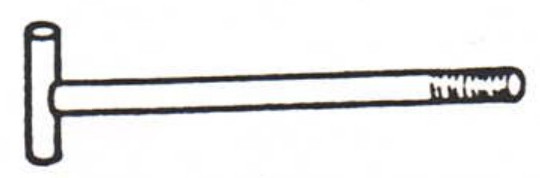
\includegraphics[width=4cm]{images/chapter7/tool_pull_rod_m5.jpg}} 
      & Pull rod with thread "M5" 
      & Page 7.35-1 \\
    \hline

    2 & \raisebox{-\height}{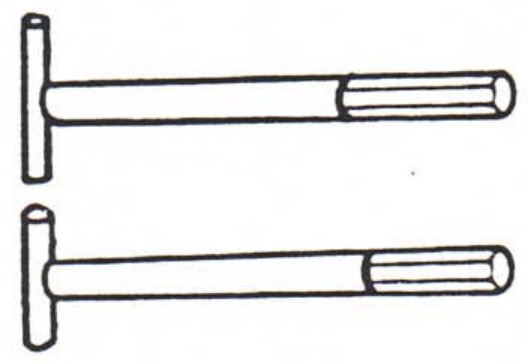
\includegraphics[width=4cm]{images/chapter7/tool_socket_wrench_5_6mm.jpg}} 
      & Socket wrench 5 mm and 6 mm 
      & Page 7.35-1 \\
    \hline

    3 & \raisebox{-\height}{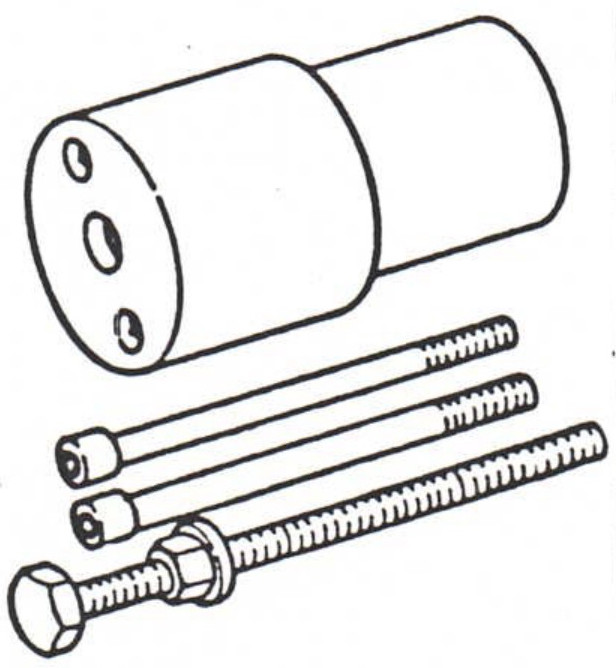
\includegraphics[width=4cm]{images/chapter7/tool_tacho_anchor_puller.jpg}} 
      & Puller, tachometer anchor 
      & Page 7.60-1 \\
    \hline
\end{longtable}

\setsectiontitle{Adjusting the Gibs}
\setrevision{7631}

\setcounter{section}{30}

\textbf{The guide play on the X, Y, and Z axes} (cross slide, vertical clamping table, and spindle stock) is factory-set to \textbf{0.003 - 0.005 mm}.  
If, after an appropriate break-in period,\\ a significant increase in this value is observed, an adjustment is necessary.

The play adjustment on the linear guides is performed using gibs with a \textbf{lead ratio of 1:130.5}.  
Shortening the adjustment bushing by \textbf{0.13 mm} results in a play reduction of \textbf{0.001 mm}\footnotemark[1].

\textbf{The gibs must not be set too tight!}  
After adjustment, the cross slide and spindle stock must move evenly and backlash-free.

\subsubsection*{Adjustment Procedure}
\begin{itemize}
    \item Loosen the \textbf{hex socket screw} \circled{1}.
    \item Remove the \textbf{adjustment bushing} \circled{2}.
    \item Shorten the \textbf{adjustment bushing} \circled{2} by the required amount and reinstall.
    \item Tighten the \textbf{hex socket screw} \circled{1}.
\end{itemize}

\begin{figure}[H]
    \centering
    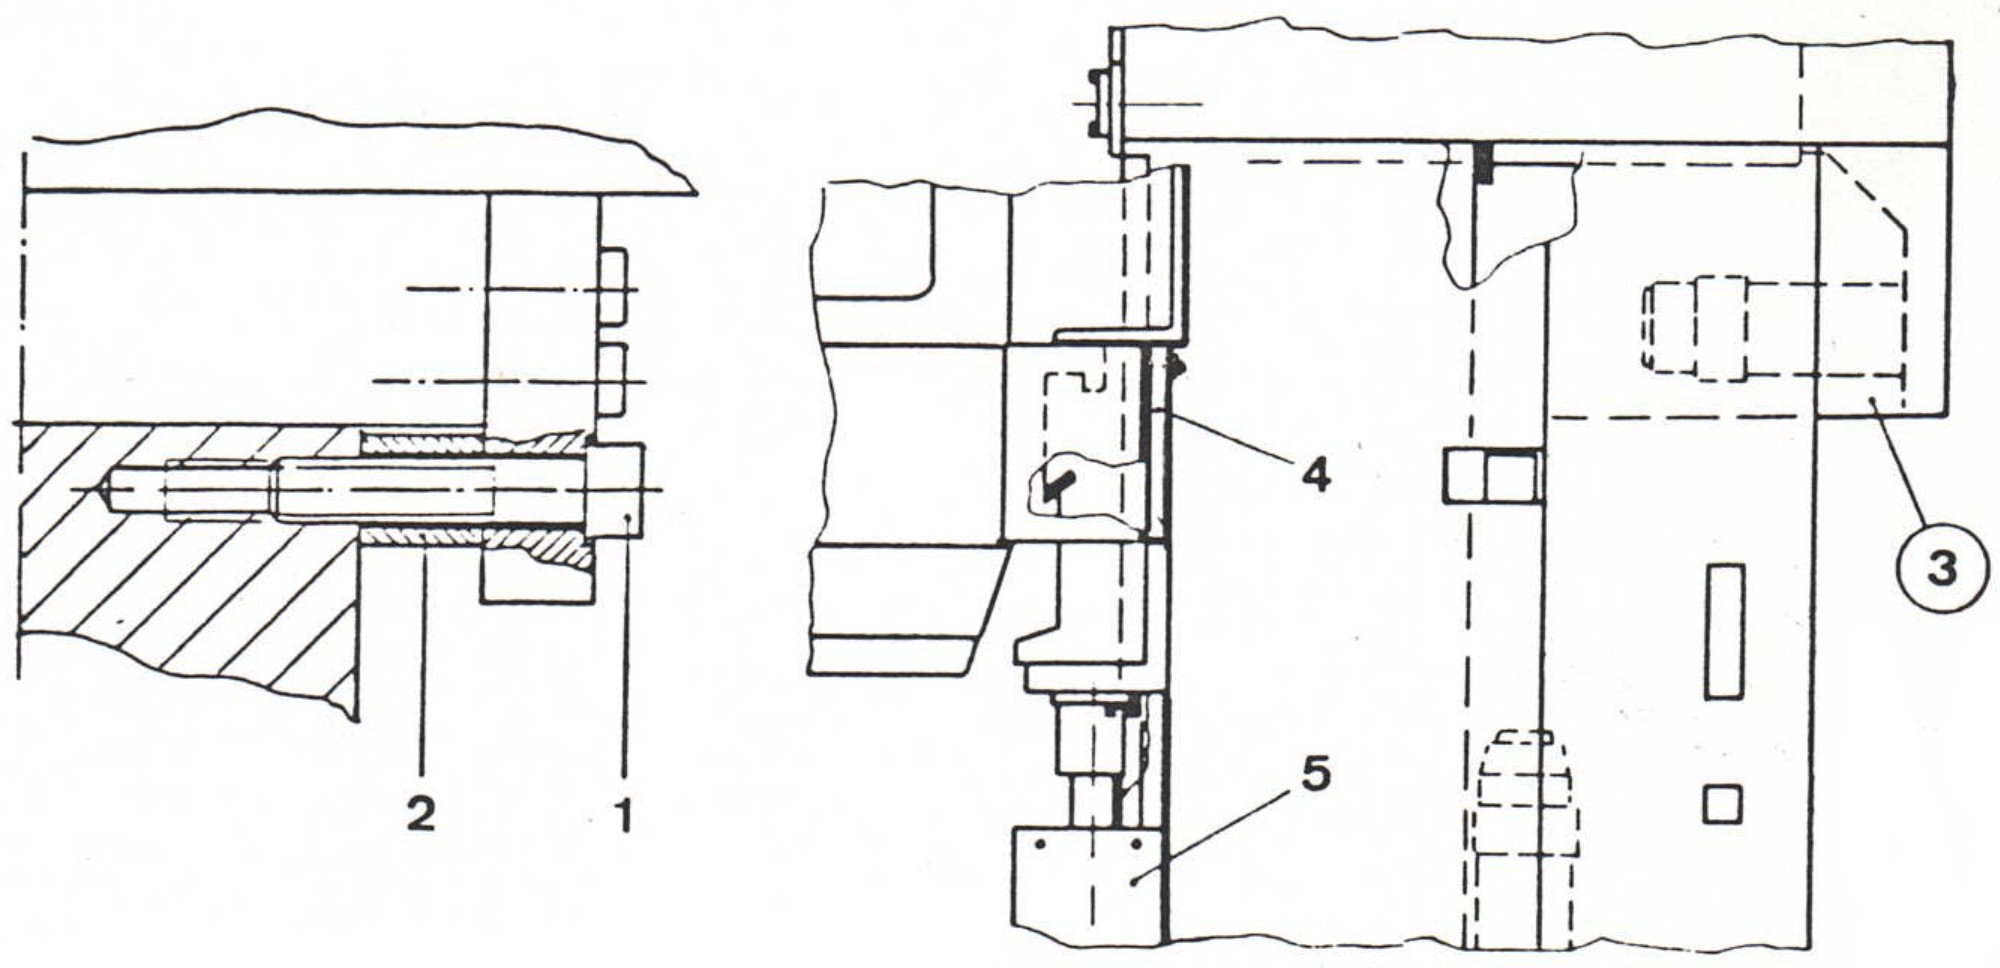
\includegraphics[width=0.8\textwidth]{images/chapter7/gib_adjustment_diagram.jpg}
    \label{fig:gib_adjustment}
\end{figure}

\textbf{Gib access points:}
\begin{itemize}
    \item \textbf{\underline{X-Axis:}} After removing the left rear cover plate \circled{4} on the cross slide.
    \item \textbf{\underline{Y-Axis:}} After removing the \textbf{telescopic cover} \circled{5} under the cross slide.
    \item \textbf{\underline{Z-Axis:}} After removing the rear cover \circled{3} on the column (see page 7.10-1).
\end{itemize}

\footnotetext[1]{Coordinate axes and movement directions can be found on page 2.03-1.}

\setsectiontitle{Guideway Wiper Maintenance}

\setcounter{section}{31}

The wipers must be checked for proper function at \textbf{1000-hour intervals}.

\subsubsection*{Checking the Wipers}
\begin{itemize}
    \item Remove the \textbf{wiper}.
    \item Clean the \textbf{wiper}.
\end{itemize}

\notebox{NOTE}{%
    If chips are pressed under the \textbf{wiper lip}, the wiper must be replaced.
}

\begin{itemize}
    \item Install a \textbf{new or cleaned wiper}, ensuring it is firmly pressed against the guideways.
    \item Apply \textbf{a thin layer of way oil} approximately \textbf{50 mm wide} onto the guideway.
    \item Move the slide \textbf{30 mm} to distribute the oil film.\footnotemark[1]
    \item The wiper is functioning correctly if it removes oil evenly along the entire guideway.
\end{itemize}

\begin{figure}[H]
    \centering
    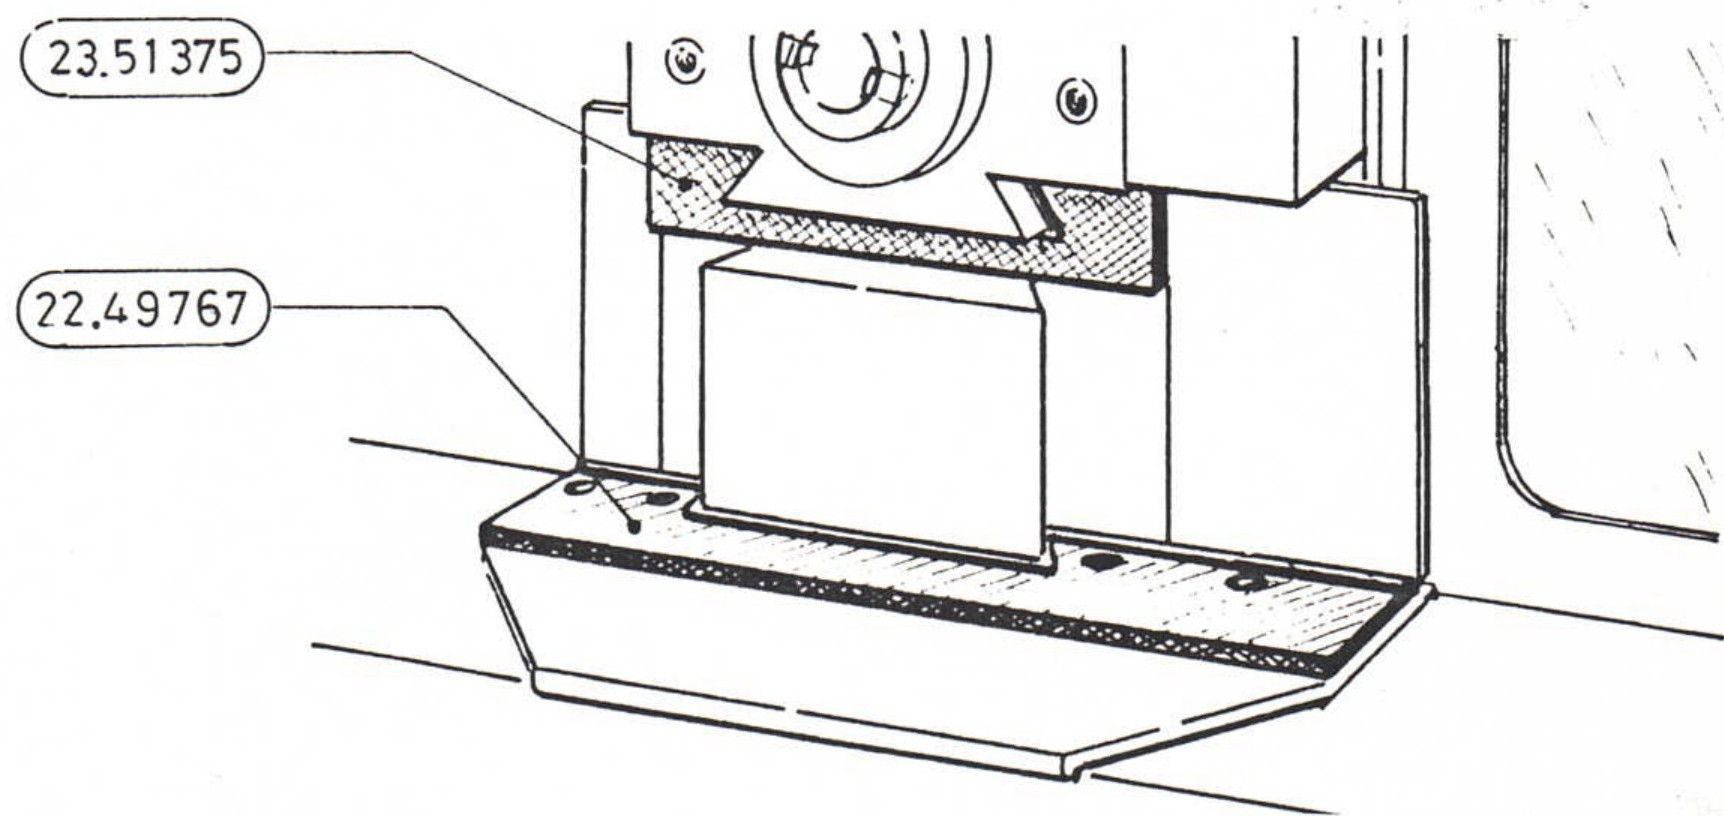
\includegraphics[width=0.8\textwidth]{images/chapter7/guideway_wiper_diagram.jpg}
    \label{fig:guideway_wiper}
\end{figure}

\notebox{WARNING}{%
    Oil mixing must be strictly avoided.
}

\footnotetext[1]{The oil used in the \textbf{central lubrication system} must be used (see page 7.06-1, \enquote{Lubricant Recommendations}).}


\setsectiontitle{Replacing the Feed Drive Timing Belt}
\setrevision{5628}

\setcounter{section}{33}

\subsection*{Feed Drive X-Axis}

\begin{itemize}
    \item Switch off the main switch \textbf{Q1} on the control cabinet.  
          To prevent accidental reactivation, the main fuses can be removed from the control cabinet.
    \item Loosen the \textbf{socket head screws \circled{1}}.
    \item Move the \textbf{motor \circled{3}} toward the lead screw so that the \textbf{timing belt \circled{5}} can be removed from the \textbf{motor shaft \circled{2}}.
    \item Remove the \textbf{screws \circled{7}} and take off the \textbf{cover \circled{4}}.
    \item Remove the old \textbf{timing belt \circled{5}}. Place a new \textbf{timing belt} onto the \textbf{drive pulley \circled{6}}.
    \item Fit the \textbf{timing belt \circled{5}} onto the \textbf{motor shaft \circled{2}}, attach the belt, and tension it by tightening the \textbf{socket head screws \circled{1}}.
    \item Reinstall the \textbf{cover \circled{4}}.
\end{itemize}

\begin{figure}[H]
    \centering
    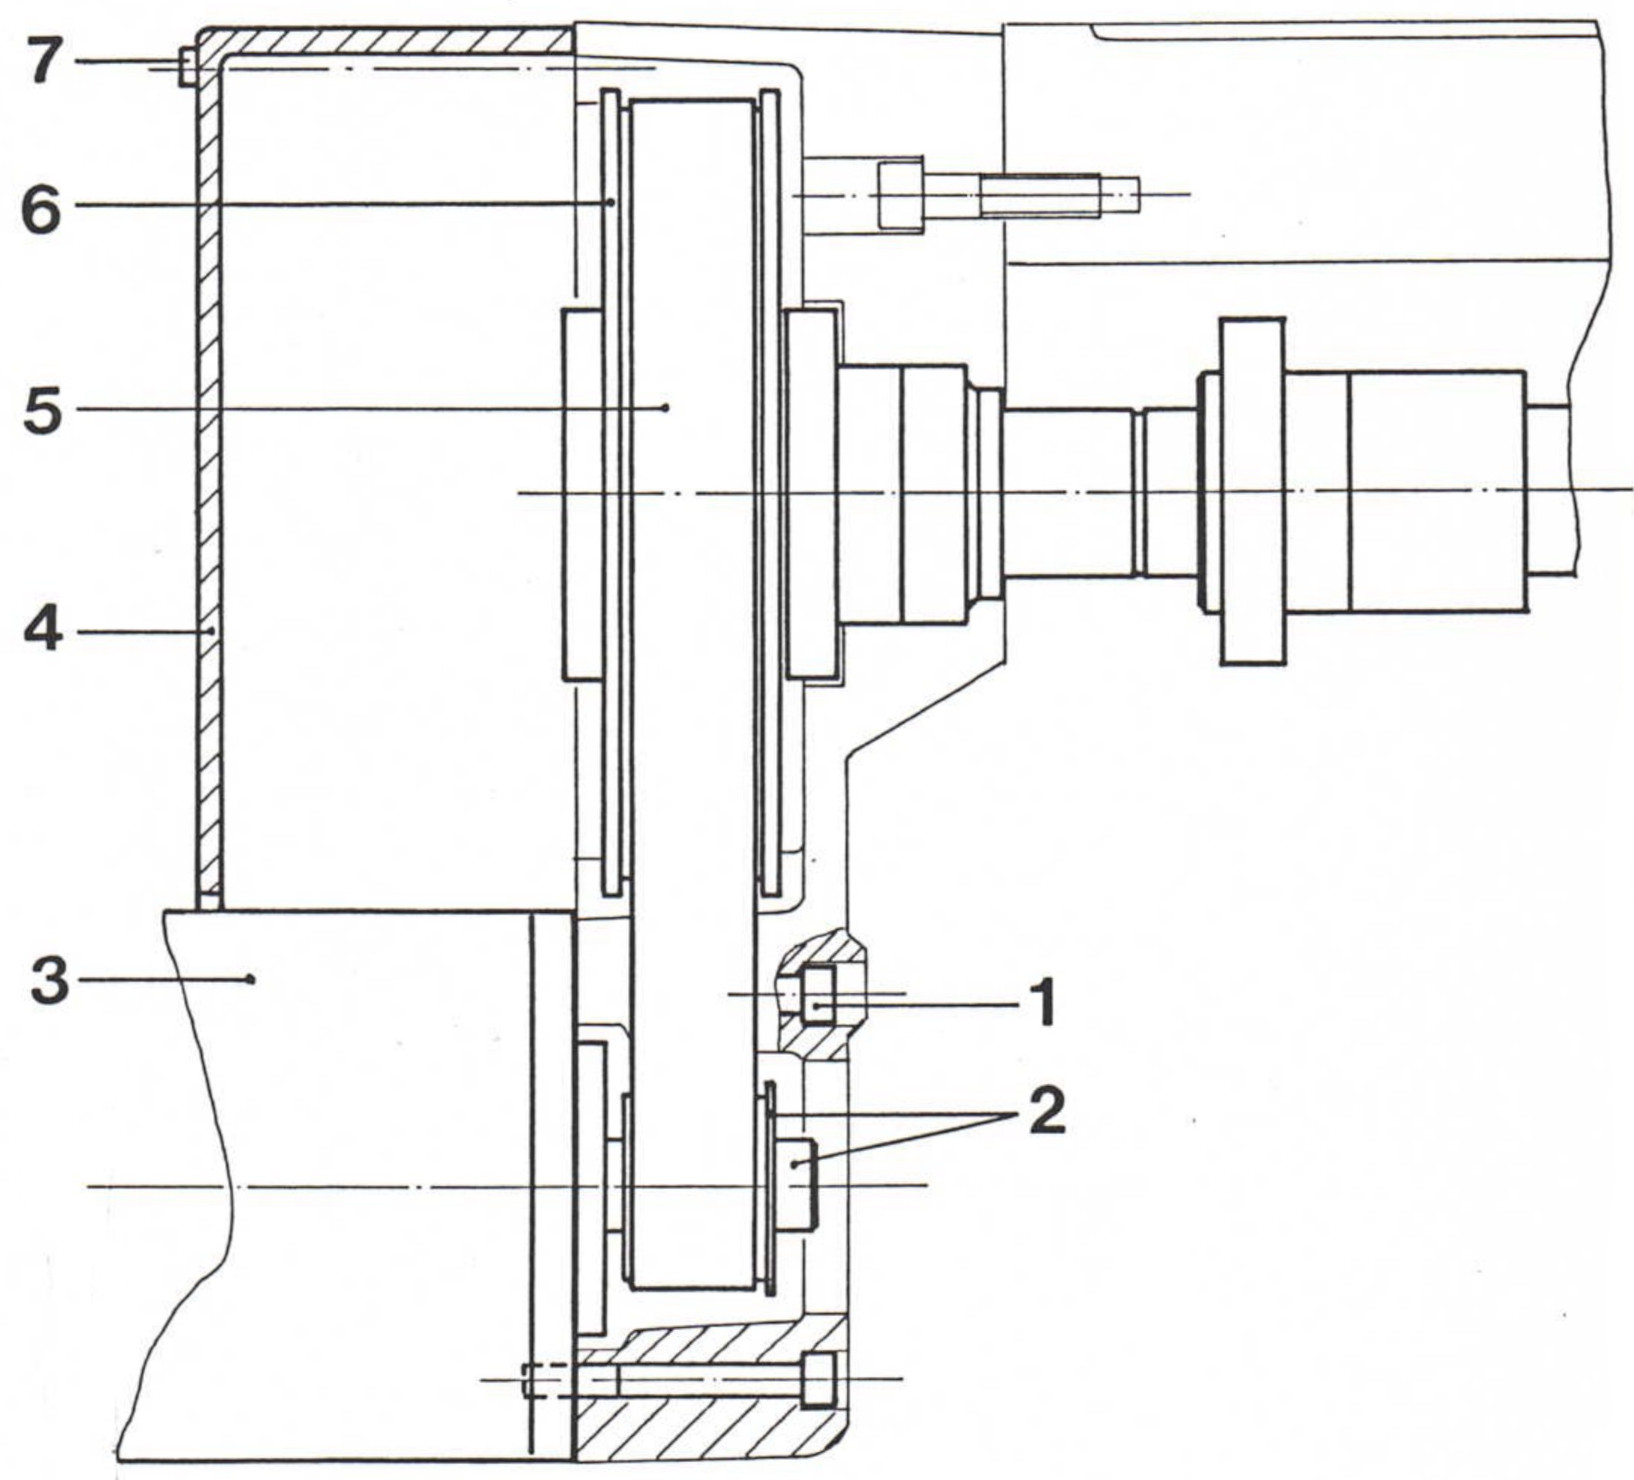
\includegraphics[width=0.8\textwidth]{images/chapter7/timing_belt_replacement.jpg}
    \label{fig:timing_belt_replacement}
\end{figure}

\newpage
\subsection*{Feed Drive Y-Axis}
\setrevision{7631}

\begin{figure}[H]
    \centering
    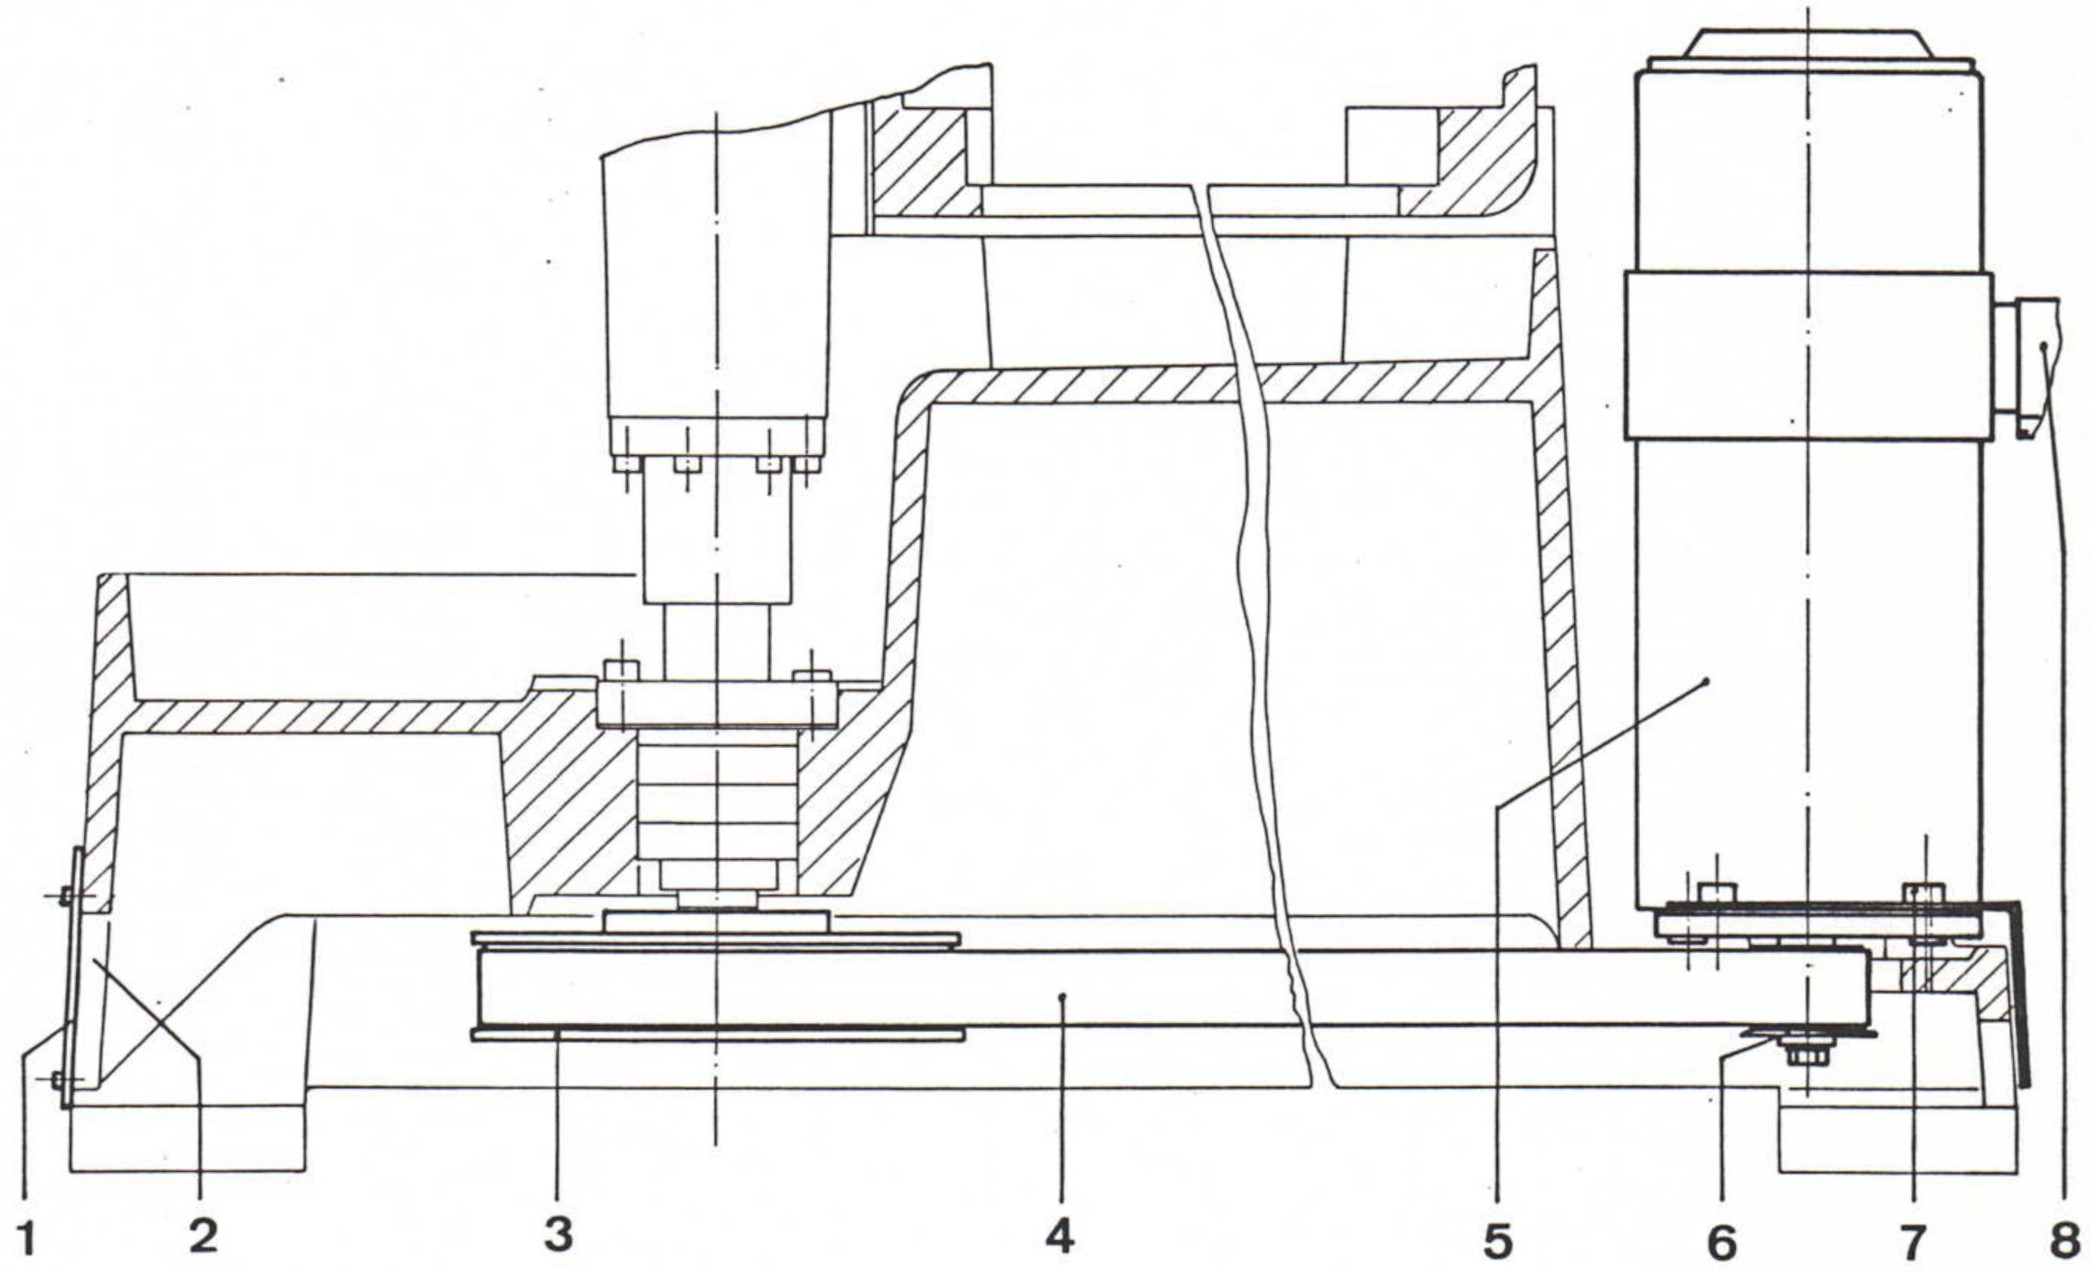
\includegraphics[width=0.8\textwidth]{images/chapter7/timing_belt_replacement_y_axis.jpg}
    \label{fig:timing_belt_replacement_y_axis}
\end{figure}

\begin{itemize}
    \item Move the \textbf{cross slide} to the upper end position and secure it.
    \item Switch off the main switch \textbf{Q1} on the control cabinet.  
          To prevent accidental reactivation, the main fuses can be removed from the control cabinet.
    \item Remove the \textbf{machine cover \circled{2}} (see page 7.10-1).
    \item Remove the \textbf{screws \circled{7}} and tilt the \textbf{motor \circled{5}} diagonally backward.
    \item Unscrew the \textbf{cover \circled{1}}.
    \item Pull out the \textbf{timing belt \circled{4}} through the front opening \textbf{\circled{2}} at the machine base.
    \item Place a new \textbf{timing belt \circled{4}} onto the \textbf{timing pulley \circled{3}} and guide it toward the motor shaft.
    \item Carefully insert the \textbf{motor \circled{5}} while fitting the \textbf{timing belt \circled{4}} onto the \textbf{timing pulley \circled{6}}.
    \item Tension the \textbf{timing belt} by shifting the \textbf{motor \circled{5}} moderately. Tighten the \textbf{screws \circled{7}}.
\end{itemize}

\notebox{NOTE}{%
    Timing belt maintenance is described on page 7.33-5.
}

\newpage
\subsection*{Feed Drive Z-Axis}

\begin{itemize}
    \item Move the \textbf{spindle head} to \textbf{Z 250}.
    \item Switch off the main switch \textbf{Q1} on the control cabinet.  
          To prevent accidental reactivation, the main fuses can be removed from the control cabinet.
    \item Remove the \textbf{screws \circled{1}} and take off the \textbf{cover \circled{1}} (see page 7.10-1).
    \item Secure the \textbf{motor \circled{5}} against tilting and loosen the \textbf{socket head screws \circled{4}}.
    \item Move the \textbf{motor \circled{5}} toward the lead screw until the \textbf{timing belt \circled{2}} can be removed from the \textbf{motor shaft \circled{3}}.
    \item Place a new \textbf{timing belt \circled{2}} onto both \textbf{timing pulleys}.
    \item Return the \textbf{motor \circled{5}} to its original position. Lightly tighten the \textbf{socket head screws \circled{4}}, check the belt tension, and then fully secure the screws.
    \item Reinstall the \textbf{cover \circled{1}}.
\end{itemize}

\begin{figure}[H]
    \centering
    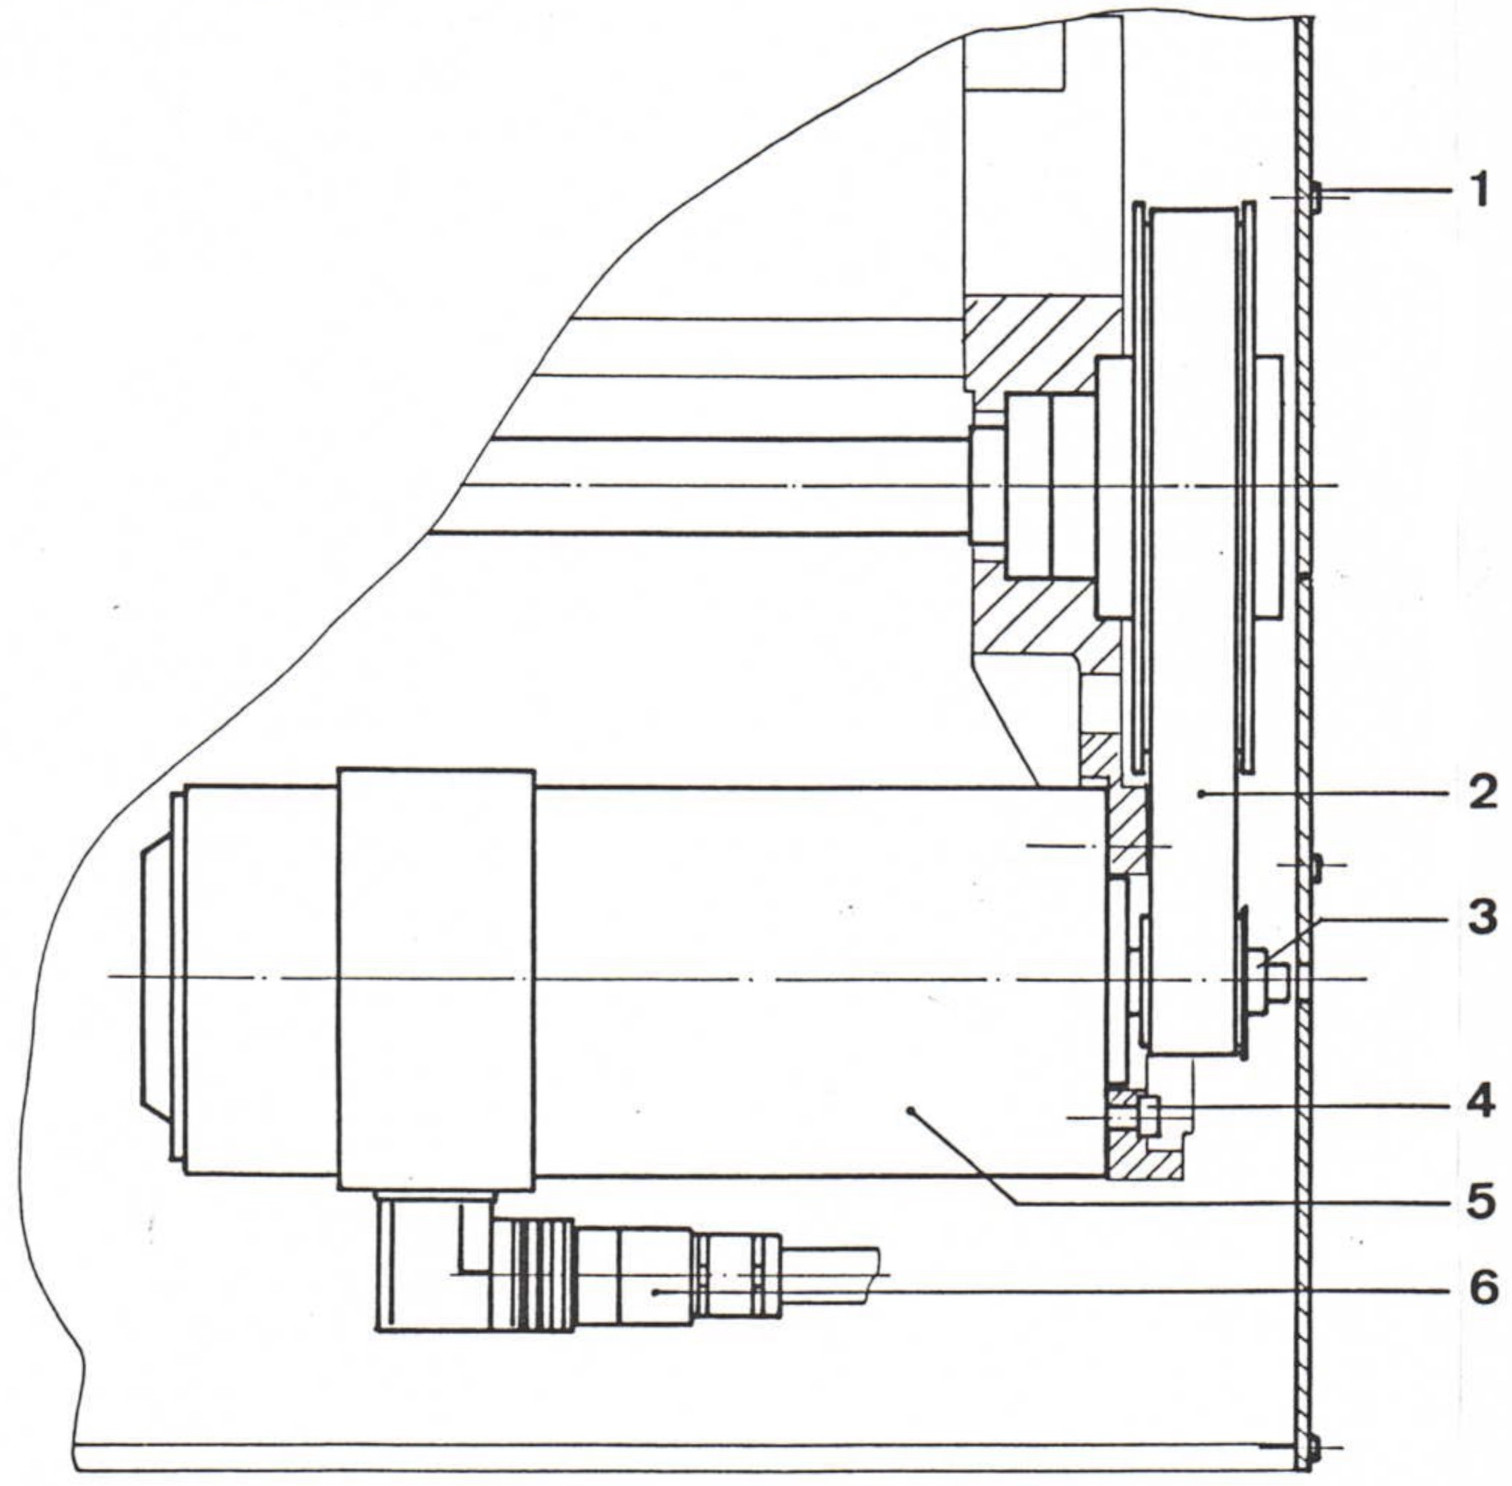
\includegraphics[width=0.8\textwidth]{images/chapter7/timing_belt_replacement_z_axis.jpg}
    \label{fig:timing_belt_replacement_z_axis}
\end{figure}

\newpage

\setcounter{page}{5}

\subsubsection*{Maintenance}
\setrevision{859}

Timing belts require no special maintenance.

Since timing belts do not experience permanent elongation during operation, a properly \\tensioned belt does not need to be retightened.  
Under no circumstances should lubricants such as grease or wax be used.

After every \textbf{1000 operating hours}:
\begin{itemize}
    \item Check for \textbf{belt wear}.
\end{itemize}

\subsubsection*{Operating Issues}

\begin{table}[H]
    \centering
    \renewcommand{\arraystretch}{1.2}
    \begin{tabular}{|p{0.35\textwidth}|p{0.30\textwidth}|p{0.30\textwidth}|}
        \hline
        \textbf{Symptom} & \textbf{Cause} & \textbf{Solution} \\
        \hline
        Excessive wear on the belt's tooth flanks. & Too low or too high belt tension. & Increase or decrease tension. \\
        \hline
        Excessive wear at the root of the belt teeth. & Too high belt tension. & Decrease tension. \\
        \hline
        Shearing of belt teeth. & Too low belt tension. & Increase tension. \\
        \hline
        Excessive running noise. & Too high belt tension. & Decrease tension. \\
        \hline
        Excessive heating. & Too low belt tension, excessive slip. & Increase tension. \\
        \hline
    \end{tabular}
\end{table}

\setsectiontitle{Installation and Maintenance of the Poly-V Belt}

\subsubsection*{Installation}

\begin{itemize}
    \item Reduce the distance between the \textbf{pulleys} sufficiently so that the \textbf{poly-V belt} can be easily placed without tension.
    \item Place the \textbf{poly-V belt} onto the pulleys.
    \item Align the \textbf{grooves} of the pulleys so they are flush.
    \item Align the \textbf{motor shaft} precisely parallel to the spindle head.  
          The allowable parallelism deviation for the drive axes is max. \textbf{$\pm$ 1°}.
    \item Pre-tension the \textbf{poly-V belt} sufficiently.  
          To do this, loosen the upper nuts on the \textbf{motor mounting bolts} and adjust the lower nuts evenly.
\end{itemize}

\notebox{WARNING}{%
    Ensure that the pulley grooves remain aligned and that the shafts are parallel during installation.
}

\begin{itemize}
    \item Tighten the \textbf{upper nuts} on the motor mounting bolts.
    \item After a short period of operation under load, check the \textbf{belt tension} and adjust if necessary.
\end{itemize}

\subsubsection*{Checking Belt Tension}

The pre-tension of the poly-V belt affects belt wear, running smoothness, drive efficiency, and the service life of the bearings.  
It is recommended to check the belt tension as follows:

\begin{minipage}{0.65\textwidth}
\begin{itemize}
    \item At \textbf{half the drum length}, place a caliper gauge lightly and measure dimension \textbf{A}.
    \item Compress the \textbf{belt strands} with the caliper gauge until firm resistance is felt.
    \item Measure the resulting dimension \textbf{B}.
    \item A \textbf{new poly-V belt} is correctly tensioned when the difference between \textbf{A and B} is approx. \textbf{3.5 - 4 mm}\footnotemark[1].
\end{itemize}
\end{minipage}
\hfill
\begin{minipage}{0.3\textwidth}
    \centering
    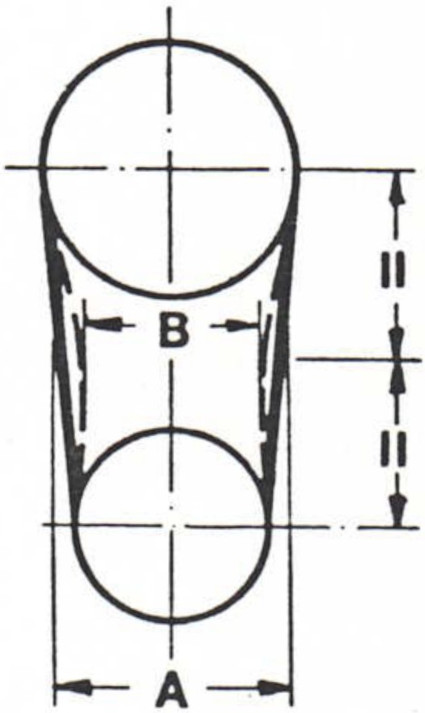
\includegraphics[width=\textwidth]{images/chapter7/poly_v_belt_tension_diagram.jpg}
\end{minipage}

\footnotetext[1]{If a previously used belt is reinstalled, the difference \textbf{A - B} should be approx. \textbf{5 - 6 mm}.}

\newpage

\subsection*{Maintenance}

Poly-V belts require no special maintenance.

\notebox{WARNING}{%
    Under no circumstances should lubricants such as grease or wax be used.
}

After every \textbf{1000 operating hours}:
\begin{itemize}
    \item Check the \textbf{belt tension} (see page 7.34-1).
    \item Inspect for \textbf{belt wear}.
\end{itemize}

\subsection*{Operating Issues}

\begin{table}[H]
    \centering
    \renewcommand{\arraystretch}{1.2}
    \begin{tabular}{|p{0.35\textwidth}|p{0.30\textwidth}|p{0.30\textwidth}|}
        \hline
        \textbf{Symptom} & \textbf{Cause} & \textbf{Solution} \\
        \hline
        Excessive wear on the belt ribs. & Too low belt tension. & Increase tension. \\
        \cline{2-3}
        & Pulley grooves are misaligned, shafts are not parallel. & Carefully align pulleys and shafts. \\
        \hline
        Uneven wear on the belt ribs. & Pulley grooves are misaligned, shafts are not parallel. & Carefully align pulleys and shafts. \\
        \hline
        Excessive running noise. & Too high belt tension. & Decrease tension. \\
        \cline{2-3}
        & Pulley grooves are misaligned, shafts are not parallel. & Carefully align pulleys and shafts. \\
        \hline
        Excessive heating. & Frequent or prolonged belt slippage. & Increase tension. \\
        \hline
    \end{tabular}
\end{table}

\setsectiontitle{Adjusting the Collet for Automatic Tool Clamping}
\setrevision{5628}

The adjustment process differs for the vertical and horizontal work spindles.  
The setting dimension is measured and adjusted only in the \textbf{release position}.

\subsection*{Prerequisites}

\begin{enumerate}
    \item The \textbf{indicator button {3SH1}} on the command station is pressed (hydraulics engaged).\footnotemark[1]
    \item The \textbf{TOOL UNCL} button on the control panel is pressed (tool clamp released).\footnotemark[1]
    \item The \textbf{tool} has been removed from the work spindle.
\end{enumerate}

\subsection*{Adjustment Procedure for the Vertical Spindle Collet}

\begin{itemize}
    \item Loosen the \textbf{threaded piece \circled{1}} with a \textbf{5 mm hex key} until a firm stop is felt.
    \item Screw the \textbf{pull rod "M5"} into the \textbf{locking piece \circled{2}} and pull it out until it reaches a stop. Remove the pull rod.
    \item Turn the \textbf{collet holder \circled{3}} using a \textbf{6 mm hex key} in or out until the setting dimension \textbf{"A"} is reached.
    \item Slightly rotate the \textbf{locking piece \circled{2}} left or right while engaging the \textbf{pull rod "M5"} into the \textbf{12-point socket \circled{4}} and fully pressing it in.
    \item Tighten the \textbf{threaded piece \circled{1}} with a \textbf{5 mm hex key} until it reaches a firm stop.
    \item Check the \textbf{setting dimension "A"} and correct if necessary.
\end{itemize}

\begin{figure}[H]
    \centering
    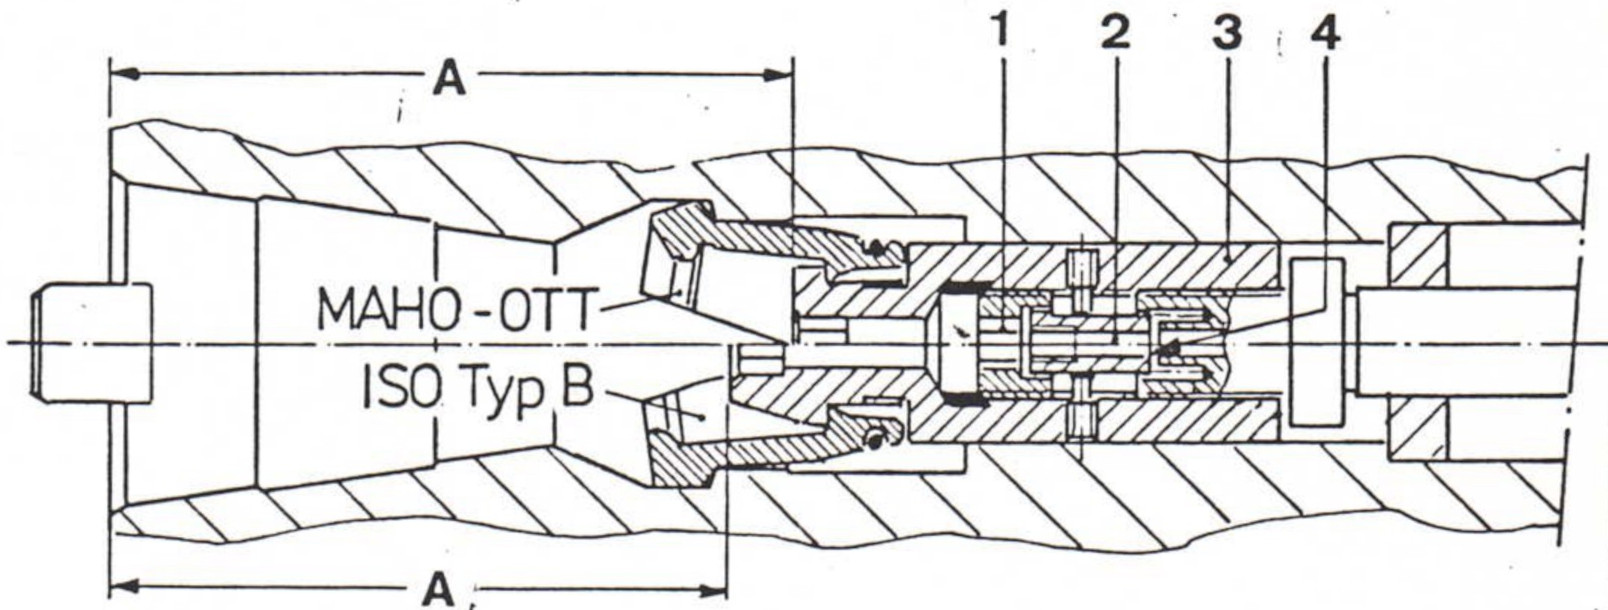
\includegraphics[width=0.8\textwidth]{images/chapter7/collet_adjustment.jpg}
    \label{fig:collet_adjustment}
\end{figure}

\footnotetext[1]{Only required for hydraulic tool clamping systems.}

\newpage

\subsection*{Adjustment Procedure for the Horizontal Spindle Collet}

\begin{itemize}
    \item Loosen the \textbf{threaded pin \circled{5}}.
    \item Adjust the \textbf{collet holder \circled{6}} using a screwdriver, turning it in or out until the setting dimension \textbf{"A"} is reached.
    \item Secure the \textbf{collet holder \circled{6}} by tightening the \textbf{hex screw \circled{5}}.
\end{itemize}

\begin{minipage}{0.5\textwidth}
    \centering
    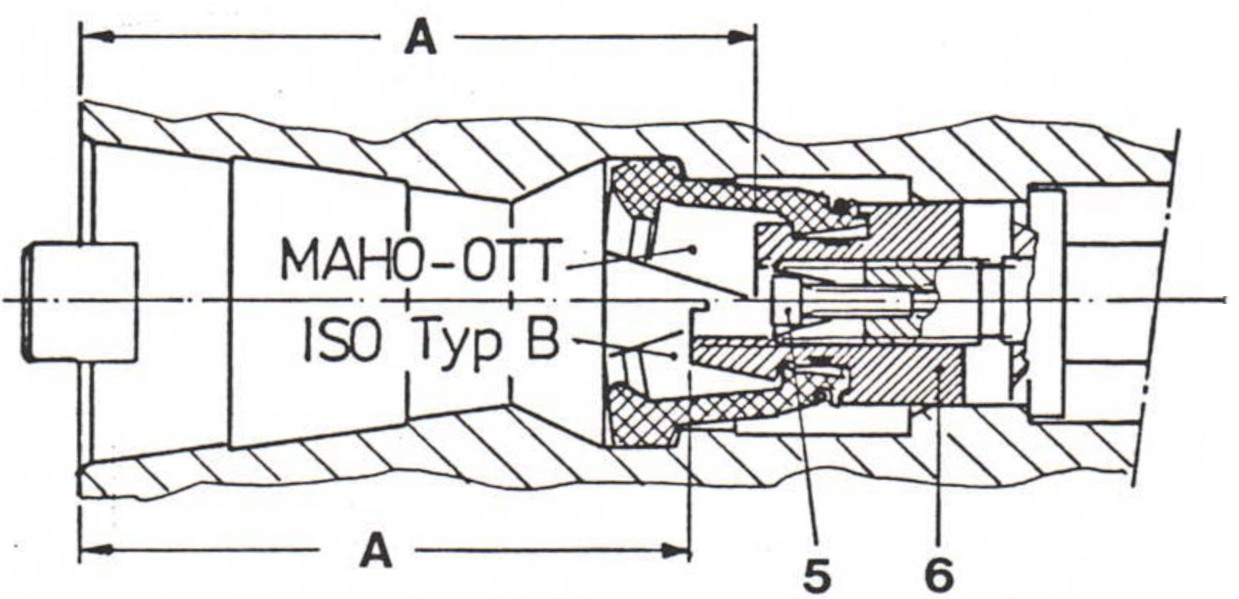
\includegraphics[width=\textwidth]{images/chapter7/collet_adjustment_horizontal.jpg}
\end{minipage}
\hfill
\begin{minipage}{0.5\textwidth}
    \centering
    \renewcommand{\arraystretch}{1.5} % Adjust row height
    \begin{tabular}{|c|c|c|}
        \hline
        & \multicolumn{2}{c|}{A} \\ \hline
        Spannzange & MAHO/OTT & \shortstack{\rule{0pt}{1.2em} ISO7388 \\ TYP B} \\ \hline
        ISO 40 & 91,4 & 82,7 \\ \hline
    \end{tabular}
\end{minipage}

\subsubsection*{Released State}

\begin{itemize}
    \item Insert the \textbf{tool} into the work spindle and press the \textbf{TOOL UNCL} button (the tool is clamped).\footnotemark[1]
    \item Press the \textbf{TOOL UNCL} button again (the tool clamp is released) and remove the tool from the spindle.
\end{itemize}

\notebox{NOTE}{%
    If the tool scrapes against the collet while being removed from the spindle, the \textbf{collet holder \circled{3}} must be adjusted further outward.  
    In this case, the setting dimension \textbf{"A"} may deviate by a maximum of \textbf{0.5 mm}.
}

\footnotetext[1]{Position and function of the control elements on the command station can be found on page 2.04-1 and section 10.7 of the CNC 432 control manual.}
\footnotetext[2]{Special tools for maintenance and servicing are listed on page 7.23-1.}

\setsectiontitle{Adjustment Work on the Universal Rotary Table}
\setrevision{8627}
\setcounter{section}{40}

\begin{figure}[H]
    \centering
    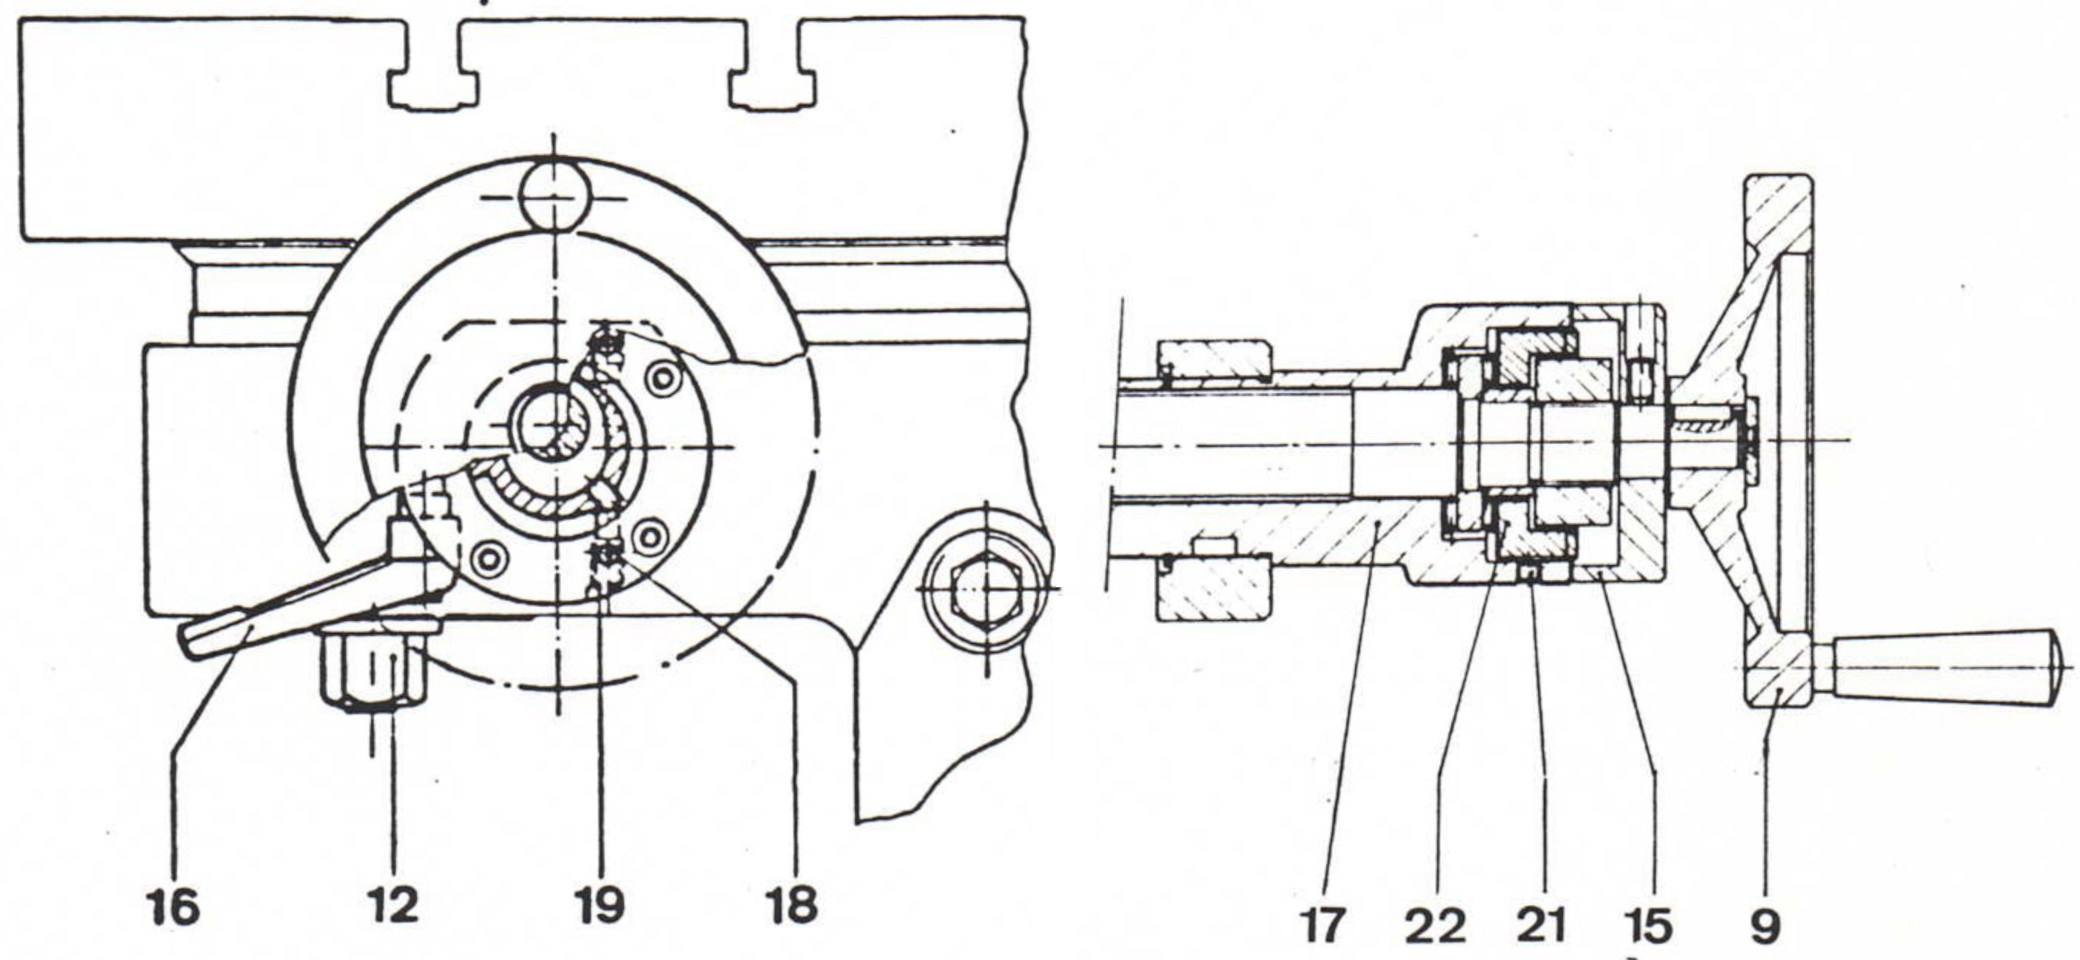
\includegraphics[width=0.9\textwidth]{images/chapter7/rotary_table_adjustment.jpg}
    \label{fig:rotary_table_adjustment}
\end{figure}

\subsection*{Checking the Backlash of the Indexing Worm}

\begin{itemize}
    \item Clamp the \textbf{table plate} and tighten the \textbf{clamping nuts \circled{12}}.
    \item Loosen the \textbf{clamping lever \circled{16}} and rotate the \textbf{eccentric bushing \circled{17}} to the right until it reaches a stop, bringing the \textbf{indexing worm} into engagement. Tighten the \textbf{clamping lever \circled{16}} again.
    \item Rotate the \textbf{handwheel \circled{9}} with moderate force.  
          A maximum \textbf{"free play"} of \textbf{10 mm} at the outer edge of the handwheel bulge is permissible.  
          If the backlash exceeds this, it must be \\readjusted.
\end{itemize}

\subsection*{Adjusting the Backlash of the Indexing Worm}

\begin{itemize}
    \item Loosen the \textbf{threaded pin \circled{18}}.
    \item Turn the \textbf{threaded pin \circled{19}} counterclockwise by approximately \textbf{10°}.
    \item Tighten the \textbf{threaded pin \circled{18}} again.
    \item Loosen the \textbf{clamping lever \circled{16}} and rotate the \textbf{eccentric bushing \circled{17}} fully to the right until it reaches a stop, further engaging the \textbf{indexing worm}. Tighten the \textbf{clamping lever \circled{16}} again.
    \item Recheck the backlash of the indexing worm.
\end{itemize}

\notebox{NOTE}{%
    If the \textbf{handwheel \circled{9}} can still rotate freely by more than \textbf{10 mm},  
    the axial bearing clearance of the indexing worm must be adjusted.
}

\newpage

\subsection*{Adjusting the Axial Bearing Clearance of the Indexing Worm}

\begin{itemize}
    \item Loosen the \textbf{threaded pin \circled{21}}.\footnotemark[1]
    \item Rotate the \textbf{locking ring \circled{22}} clockwise while simultaneously turning the \textbf{worm shaft \circled{23}}, eliminating the axial bearing clearance.
    \item Tighten the \textbf{threaded pin \circled{21}} again.
\end{itemize}

\subsection*{Adjusting the Adjustable Clamping Lever}

\begin{itemize}
    \item For design reasons, the \textbf{swivel angle of the clamping lever \circled{16} is limited}.
    \item If, due to wear, the \textbf{clamping lever \circled{16}} can no longer be fully swiveled into position where the required clamping force is achieved, it must be readjusted.
    \item To adjust, pull the lever handle back **against the force of a spring** in an axial direction; this disengages the handle from the \textbf{serrated engagement} on the clamping lever.
    \item Swivel the lever handle to the desired angle.
    \item Upon release, the lever handle will re-engage in the serrated engagement.
\end{itemize}

\footnotetext[1]{For certain table designs, remove the \textbf{handwheel \circled{9}} and \textbf{ring \circled{15}} beforehand.}

\setsectiontitle{Maintenance of DC Motors for the Feed Drive}
\setrevision{7631}

\setcounter{section}{60}

\subsection*{Removal and Installation Instructions for the Tachometer Rotor}

\notebox{WARNING}{%
    When working on the tachometer rotor, ensure that the winding is not damaged.  
    Additionally, it is not permitted to loosen the tachometer's field windings in the yoke,  
    as this would cause a shift of the neutral zone, which cannot be corrected easily.
}

If a tachometer rotor with a serial number of 3051 or higher replaces a\\tachometer from serial numbers up to 3050,  
the changed tachometer polarity requires swapping the red and blue terminal wires on the side-mounted circuit board.

\subsubsection*{1. Removing the Tachometer Rotor}

\begin{itemize}[itemsep=1pt,parsep=0pt]
    \item Remove the \textbf{cover \circled{1}} and pull off the \textbf{housing \circled{2}}.
    \item Remove the \textbf{carbon brushes \circled{8}}, marking them individually  
          to ensure they are later reinstalled in the same holder and mounting position.  
          See page 7.60-2 for details.
    \item Secure the \textbf{pulling device \circled{5}} to the \textbf{tachometer rotor \circled{7}} using the \textbf{screws \circled{4}}.\footnotemark[1]
    \item Pull off the \textbf{tachometer rotor \circled{7}} from the \textbf{motor shaft \circled{6}},  
          supporting it against the motor shaft while turning the \textbf{screw \circled{3}} clockwise.
\end{itemize}

\subsubsection*{2. Installing the Tachometer Rotor}

\begin{itemize}[itemsep=1pt,parsep=0pt]
    \item Slide a \textbf{new tolerance ring \circled{9}} onto the \textbf{motor shaft \circled{6}}.  
          Each tolerance ring can only be used once.
    \item Attach the \textbf{pulling device \circled{5}} (without the \textbf{screw \circled{3}})  
          to the new tachometer rotor and slide it onto the \textbf{motor shaft}.  
          Turn the \textbf{screw \circled{11}} into the motor shaft.
    \item Tighten the \textbf{rotor} by turning the \textbf{nut \circled{10}} clockwise until it reaches a stop.
    \item Reinstall the \textbf{carbon brushes \circled{8}}, following the guidelines on page 7.60-2.
\end{itemize}

\begin{figure}[H]
    \centering
    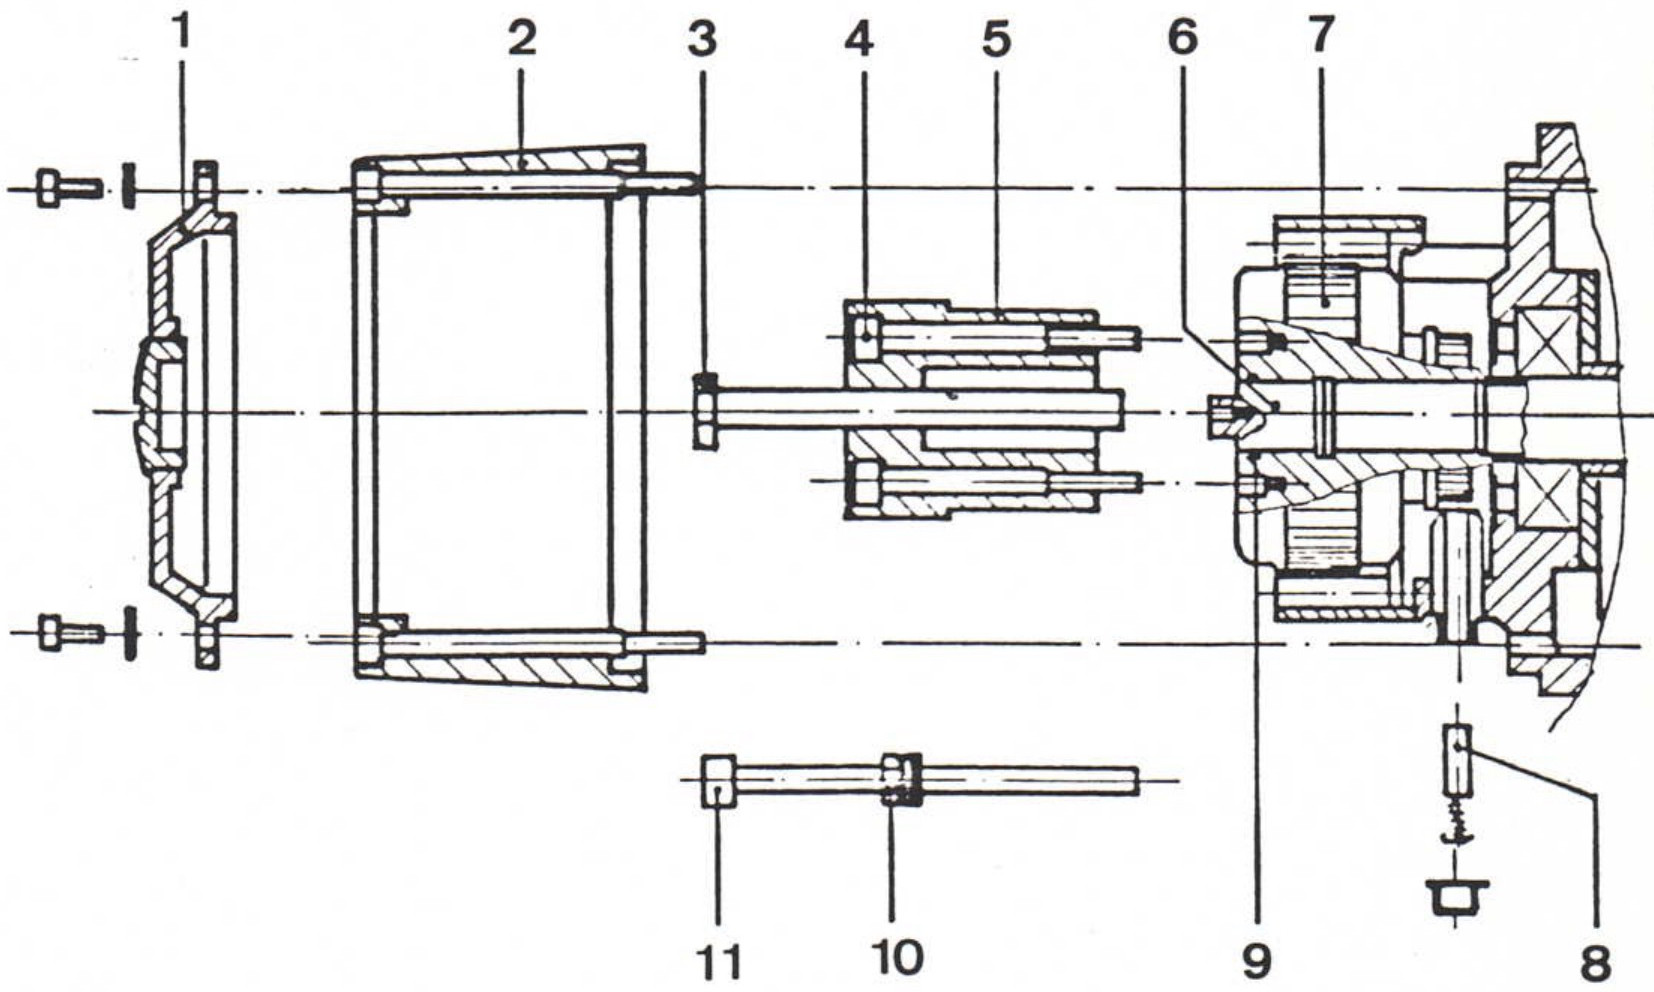
\includegraphics[width=0.55\textwidth]{images/chapter7/tachometer_rotor_replacement.jpg}
    \label{fig:tachometer_rotor_replacement}
\end{figure}

\footnotetext[1]{Special tools for maintenance and servicing are listed on page 7.23-1.}

\newpage

\subsection*{Inspection and Replacement of Carbon Brushes}
\setrevision{859}

The carbon brushes in the motor and tachometer are subject to wear.  
They must be checked regularly for smooth movement, wear, and uniform spring\\ tension.  
If they approach the wear limit shown below, they must be replaced.
Brush dust deposits in the collector chamber should be blown out with dry compressed air  
after removing all brushes.

Each removed carbon brush must be reinstalled in the same holder and in the same position.

It is important to ensure that the \textbf{locking caps are seated correctly} on the holders,  
as this guarantees proper contact between the spring plate and the holder.  
Brush replacement must always be carried out as a complete set.  
Only original-quality brushes should be used.


\begin{figure}[H]
    \centering
    \begin{minipage}{0.48\textwidth}
        \textbf{Motor Brushes: 106-57-42155} \\(Set of 4).  
    \end{minipage}
    \hfill
    \begin{minipage}{0.48\textwidth}
        \textbf{Tachometer Brushes: 105-251-4207} \\(Set of 4).  
    \end{minipage}

    \vspace{3pt} % Adjust spacing between text and image

    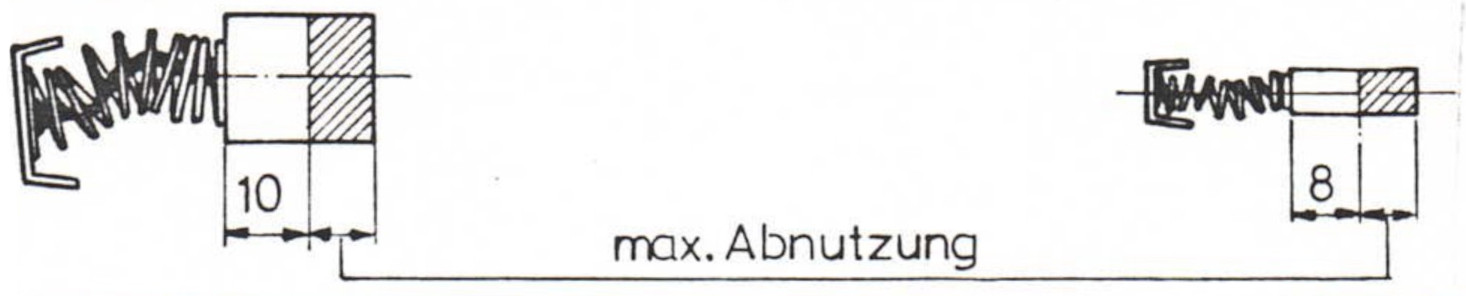
\includegraphics[width=0.8\textwidth]{images/chapter7/carbon_brushes_wear_limit.jpg}
    \label{fig:carbon_brushes_wear_limit}
\end{figure}

\begin{table}[H]
    \centering
    \renewcommand{\arraystretch}{1.2}
    \begin{tabular}{|p{0.3\textwidth}|p{0.3\textwidth}|p{0.3\textwidth}|}
        \hline
        \textbf{Maintenance Interval} & \textbf{Motor Brushes} & \textbf{Tachometer Brushes} \\
        \hline
        Machine Operation & 6 months & 6 months \\
        \hline
    \end{tabular}
\end{table}

\begin{figure}[H]
    \centering
    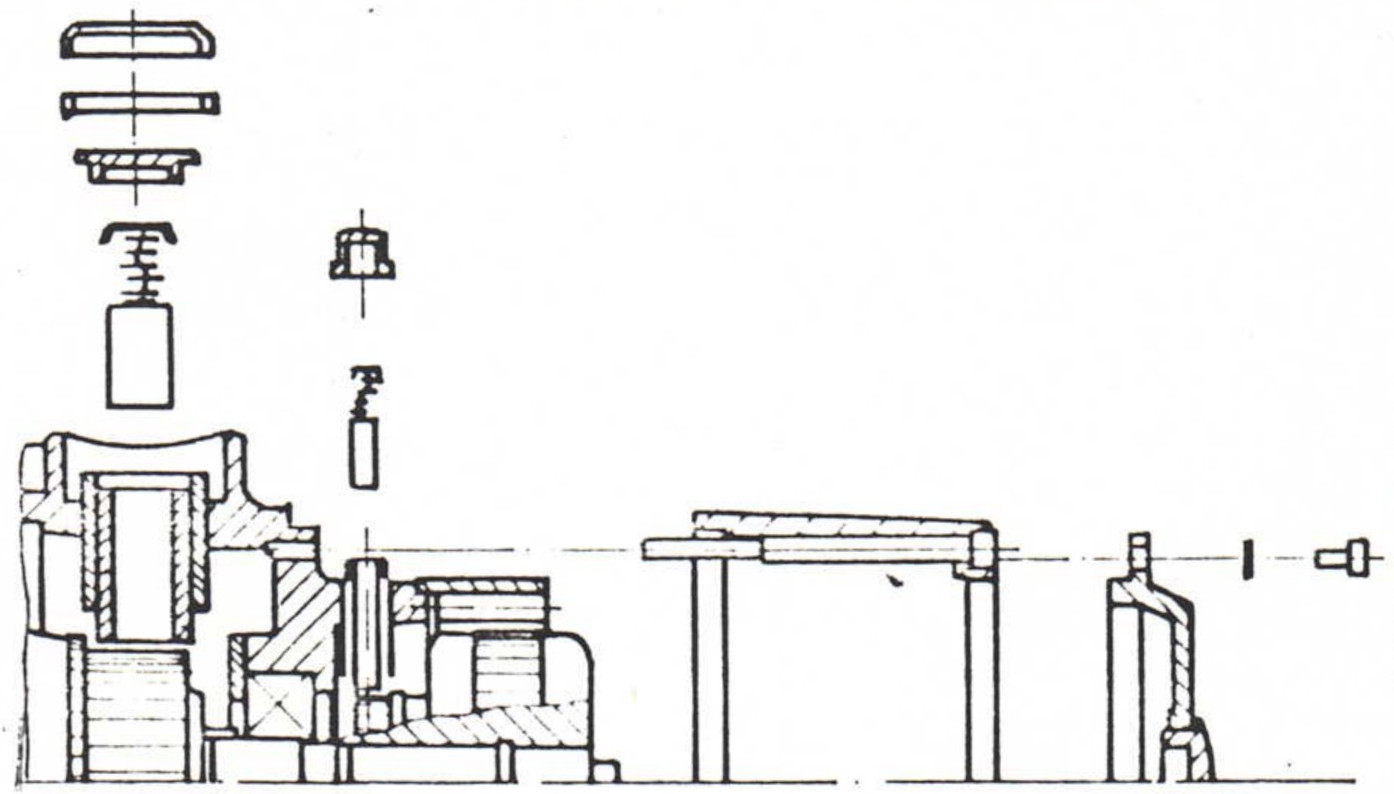
\includegraphics[width=0.7\textwidth]{images/chapter7/air_filter_assembly.jpg}
    \label{fig:air_filter_assembly}
\end{figure}

\subsection*{Inspection and Replacement of Air Filters}

Internally ventilated motors have a built-in fan with a pre-mounted air filter disk.  
This filter disk cleans the intake cooling air from solid contaminants.  
Depending on the level of contamination in the intake air, the filter must be cleaned or replaced periodically.

\newpage

\subsection*{Cleaning}

\begin{itemize}
    \setlength{\itemsep}{0pt} \setlength{\parskip}{0pt}
    \item Rinse in water (up to approx. \textbf{40°C}, optionally with mild detergents)  
          or, in extreme cases, in gasoline.
    \item Knocking out or blowing out with compressed air is also possible.
    \item \textbf{Avoid wringing!}
    \item When rinsing with water, avoid using a high-pressure water jet.
\end{itemize}

\subsection*{Important When Replacing}

The dust air side has an open structure, while the cleaning side has a closed,  
\\binder-reinforced structure.

\subsection*{Ordering Information}

Filter Mat Type P15/500, 100 Ø (Viledon).

\setsectiontitle{Maintenance of Three-Phase Motors - Main Drive}
\setrevision{7631}

\subsection*{General Maintenance}

\begin{itemize}
    \setlength{\itemsep}{0pt} \setlength{\parskip}{0pt}
    \item The three-phase motors require no special maintenance.
    \item The rolling bearings have lifetime lubrication and do not require \\relubrication.
    \item Maintenance is limited to cleaning the motor housing and adjusting the brake.
\end{itemize}

\subsection*{Cleaning the Motor Housing}

\begin{itemize}
    \setlength{\itemsep}{0pt} \setlength{\parskip}{0pt}
    \item Clean the cooling air passages, especially the spaces at the base of the cooling fins.
    \item Any accumulation of dust or other residues obstructs airflow  
          and can cause excessive \\overheating.
    \item Remove dust deposits and dirt using a \textbf{bellows blower}.
\end{itemize}

\subsection*{Adjusting the Brake}

The wear of the brake linings must be checked after every \textbf{1,000 operating hours}.  
If necessary, the air gap must be readjusted.

\begin{itemize}
    \setlength{\itemsep}{0pt} \setlength{\parskip}{0pt}
    \item Remove the \textbf{fan cover \circled{6}} and the \textbf{retaining ring \circled{7}}.
    \item Pull off the \textbf{fan \circled{5}} and remove the \textbf{dust protection ring \circled{2}}.
    \item Measure the \textbf{air gap a} at least three positions around the circumference using a feeler gauge.
    \item Loosen the \textbf{socket head screws \circled{4}} by approx. \textbf{half a turn}.
    \item Adjust the \textbf{adjusting sleeves \circled{1}} by turning them approx. \textbf{one-third of a turn},  
          then screw them into the \textbf{coil housing \circled{3}}.
    \item Tighten the \textbf{socket head screws \circled{4}}, check the \textbf{air gap \enquote{a}}, and repeat \\adjustment if necessary.
    \item Reinstall the removed components (\textbf{\circled{2}, \circled{5}, \circled{7}, \circled{6}}).
\end{itemize}

\begin{figure}[H]
    \centering
    \begin{minipage}{0.48\textwidth}
        \centering
        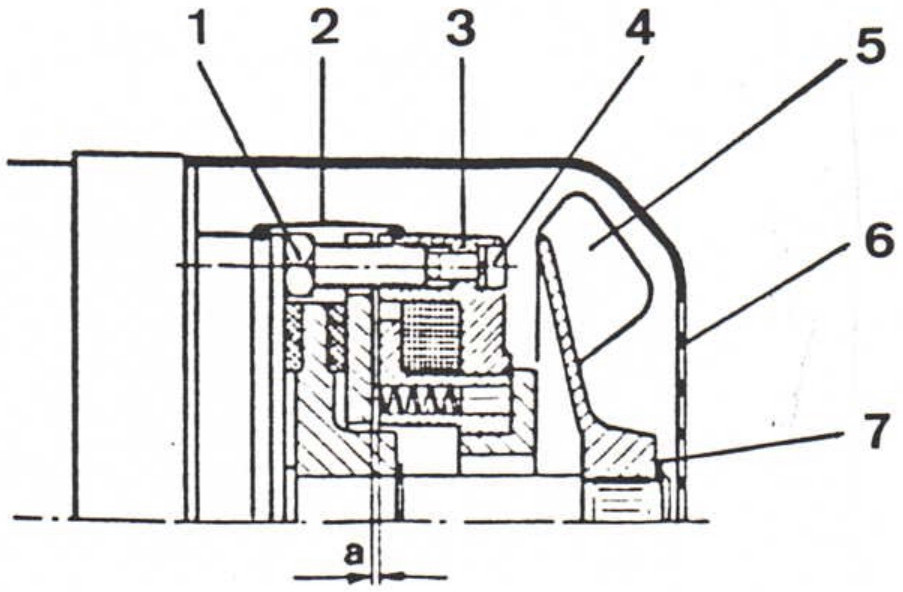
\includegraphics[width=\textwidth]{images/chapter7/brake_adjustment.jpg}
        \label{fig:brake_adjustment}
    \end{minipage}
    \hfill
    \begin{minipage}{0.48\textwidth}
        \centering
        \renewcommand{\arraystretch}{1.2}
        \begin{tabular}{|p{0.32\textwidth}|p{0.3\textwidth}|p{0.3\textwidth}|}
            \hline
            \textbf{Air Gap \enquote{a}} & \multicolumn{2}{c|}{\textbf{Machine Type}} \\
            \hline
            & \textbf{MH 400 E MH 600 E MH 800 E} & \textbf{MH 2000 C} \\
            \hline
            \textbf{Min.} & 0.3 mm & 0.4 mm \\
            \hline
            \textbf{Max.} & 1.0 mm & 1.4 mm \\
            \hline
        \end{tabular}
    \end{minipage}
\end{figure}